\documentclass[]{htwg-report}

\addbibresource{./bib/report.bib}

% abbreviations:
\newacronym{crm}{cRM}{combit Relationship Manager}
\newacronym{ll}{LL}{List \& Label}
\newacronym{CRM}{CRM}{Customer Relationship Management}
\newacronym{dsgvo}{DSGVO}{Datenschutz-Grundverordnung}
\newacronym{COM}{COM}{Component Object Model}
\newacronym{wysiwyg}{WYSIWYG}{What You See Is What You Get}
\newacronym{ssr}{SSR}{Server-Side-Rendering}
\newacronym{svn}{SVN}{Subversion}
\newacronym{cli}{CLI}{Command-Line-Interface}
\newacronym{cra}{CRA}{create-react-app}

\makeglossaries{}


\begin{document}

%% Use Roman numerals for the page numbers of the title pages and table of contents.
\frontmatter{}

%% 'reporttype' add background elements to the cover / front page
%% possible values are:
%% bachelor	--> B S C
%% master	--> M S C
%% other	--> none
\reporttype{bachelor}

\reporttypetext{Bachelorthesis}

\title{Konzipierung der Architektur einer Darstellungsschicht basierend auf aktuellen Webtechnologien im Hinblick auf eine zukünftige Anbindung an das Programm combit Relationship Manager}

\author{Jonas Reinwald}
\studentnumber{293320}
\studentemail{jonas.reinwald@protonmail.com}

\doclocation{Konstanz}
\docdate{\today}

\makecover[]

\begin{titlepage}
    \newgeometry{hscale=0.81,vscale=0.8}
    
    \AddToShipoutPicture*{\BackgroundImgTitelPage}
    
    \vspace*{12\bigskipamount}
    
    %% Print the title in HTWG-teal.
    {
        \makeatletter
        \fboxsep=0pt
        \colorbox{htwg-white}{\begin{minipage}[t]{145mm}
            \begin{flushleft}
                %% Print Report Type Text
                \color{htwg-teal}\LARGE{\@report@typetext}
                \\
                %% Print Report Title
                \color{htwg-teal}\Large\textbf{\@title}
            \end{flushleft}
        \end{minipage}}
        \makeatother
    }
    
    \bigskip
    \bigskip

    von
    %door
    
    \bigskip
    
    %% Print the name of the author.
    {
        \makeatletter
        \large\bfseries\@author{} % chktex 21
        \makeatother
    }
    
    \vfill
    
    Zur Erlangung des akademischen Grades eines

    {
        \makeatletter
        \fboxsep=0pt
        \colorbox{htwg-white}{\begin{minipage}[t]{50mm}
            \begin{flushleft}
                \vspace*{.6\bigskipamount}
                {\bfseries Bachelor of Science (B.Sc.)}
                \vspace*{.6\bigskipamount}
            \end{flushleft}
        \end{minipage}}
        \makeatother
    }
    
    
    
    an der Hochschule Konstanz für Technik, Wirtschaft und Gestaltung
    
    \vfill
    
    \begingroup
    \renewcommand*{\arraystretch}{1}
    \rowcolors{2}{white}{white}
    {
        \makeatletter
        \begin{tabular}{>{\raggedright\arraybackslash}p{3.5cm}l}
            Vorgelegt von: & Jonas Reinwald \\
                & Wessenbergstr. 13 \\
                & 78462 Konstanz \\
                & \@student@number{} (Matr.-Nr.) \\
            Erstbetreuer: & \textbf{Prof.\ Dr.\ Marko Boger} \\
            Zweitbetreuer: & \textbf{Dipl.-Inf.\ Alexander Horak} \\ 
                & combit GmbH \\
                & Untere Laube 30 \\
                & 78462 Konstanz \\
            Ausgegeben am: & 01.12.2018 \\
            Eingereicht am: & 28.02.2019 \\
        \end{tabular}
        \makeatother
    }
    \endgroup
    
    \bigskip
    
    %% reset page margins
    \newgeometry{hscale=0.7,vscale=0.8}
    \end{titlepage}


\chapter{Zusammenfassung (Abstract)}

Webapplikationen in Form von mobilen Apps, Single-Page-Applikationen, \ldots \fixme{beispiel} machen heute bereits einen sehr großen Teil häufig genutzter Software aus.
In Zukunft wird der Anteil von webbasierter Software im Vergleich zu traditioneller Software noch weiter ansteigen (\fixme{quelle}).
Auch für Unternehmen ist es langfristig wichtig diesem Trend zu folgen um Kunden flexiblere Softwarelösungen anbieten zu können und nicht den Eindruck zu erwecken man könne nicht mit modernen Entwicklungen mithalten (\fixme{formulierung}).
Die Firma combit GmbH entwickelt mit dem combit Relationship Manager eine Software für das Management von Kundenbeziehungen (Customer Relationship Management), die zum momentanen Zeitpunkt aus einer Desktopapplikation, einer Webapplikation und einer mobile Webapplikation besteht, welche unabhängig voneinander entwickelt und benutzt werden.
Im Rahmen dieser Bachelorthesis soll ein Architekturkonzept für eine einheitliche Oberfläche (ThinClient, \fixme{erklärung}) basierend auf moderner Webtechnologie erarbeitet werden, mithilfe derer die drei momentanen Ausführungen des combit Relationship Managers abgelöst werden können.

\fixme{formulierung:}
Zur Erstellung dieses Konzepts beschäftigt sich diese Arbeit unter anderem mit der Evaluierung eines geeigneten Frontend-Frameworks bzw.\ einer Frontend-Bibliothek, der Kommunikation zwischen neuem UI-Layer und Backend und der Unterstützung aller bisherigen Features der Desktopapplikation.
Zwei besonders spannende Probleme existieren hier zum einen in der Flexibilität der momentanen Oberfläche, welche von jedem Nutzer individuell anpassbar ist. Diese Flexibilität soll durch eine automatische Konvertierung zu einem von der neuen UI darstellbarem Format und weiterhin anpassbarem Format erhalten bleiben. 
Zum anderen bietet die Desktopapplikation die Möglichkeit Skripte und automatisierte Aufgaben zur Anpassung der zugrunde liegenden Daten, für Darstellungsbedingungen und weitere Zwecke direkt auf dem Client auszuführen. Das Ausführen auf dem Client ist bei Webapplikationen nicht ohne Weiteres möglich, weshalb eine andere Lösung für diese Funktionalität gefunden werden muss.


\tableofcontents

\addcontentsline{toc}{chapter}{Abbildungsverzeichnis}
\listoffigures

\renewcommand\lstlistlistingname{Quellcodeverzeichnis}
\addcontentsline{toc}{chapter}{\lstlistlistingname}
\lstlistoflistings{}

\printacronyms[style=long3colheader,title=Abkürzungsverzeichnis]

%% Use Arabic numerals for the page numbers of the chapters.
\mainmatter{}


% CHAPTERS
\chapter{Einleitung}\label{chap:introduction}

\section{Motivation}
Ein Großteil der heute genutzten Software kann über eine Weboberfläche angesprochen werden. Dies hat den Vorteil, dass keine langwierigen und komplizierten Installationen vorgenommen werden müssen und, eine bestehende Internetverbindung vorausgesetzt, die Applikation von überall erreichbar ist. Die Firma combit GmbH hat diese Entwicklung bereits früh erkannt und bietet für den combit Relationship Manager eine entsprechende Weboberfläche an. Diese existiert bereits seit etlichen Jahren und basiert, bedingt durch den damaligen Stand der Technik auf nicht mehr zeitgemäßen Technologien. Da der Fokus der Entwicklung --- bestimmt durch die Nutzung der Kunden --- auf der Desktopanwendung liegt waren auch nicht genug Ressourcen vorhanden um die Technologien nach und nach durch modernere Alternativen zu ersetzen.
Webtechnologien haben außerdem nicht nur Vorteile für ihre Nutzer, sie bringen auch einige interessante Aspekte für das Entwicklerteam mit sich. Sehr viele technische Fortschritte fanden in den letzten Jahren in diesem Bereich statt, was einem nicht nur ermöglicht moderne Projekte und Konzepte kennen zu lernen, sondern auch, dass man eine breite Auswahl für eine solide Basis des eigenen Produkts hat. Ein spezielles Beispiel für einen solchen Fortschritt sind Programme, die es einem erlauben Webseiten wie normale Programme nativ auf einem Desktopcomputer darstellen zu können. Das Ziel hierbei ist, langfristig nur noch eine einzige Version für alle Umgebungen entwickeln zu müssen, wodurch Ressourcen gespart werden können und durch den einheitlichen Fokus, so die Erwartung, ein besseres Produkt entsteht. Dieses Potential der Webtechnologien wird dadurch noch weiter gesteigert, dass durch einfache Sprachen wie HTML, CSS und JavaScript, welches nicht kompiliert werden muss und auf so gut wie jedem modernen Gerät lauffähig ist, schnelle Iterationsschritte von Software möglich sind.
Wegen der genannten Gründe wurde entschieden, das Thema Web mit einer frischen Herangehensweise, einer neuen Perspektive und modernen Technologien neu anzugehen um den combit Relationship Manager sowohl extern als auch intern noch attraktiver zu machen.

\section{Erwartete Schwierigkeiten}
Bereits im Vorfeld soll ein kleiner Überblick über die Bereiche dieser Arbeit gegeben werden, welche im Laufe der Umsetzung zu Schwierigkeiten führen könnten. Dies dient sowohl der Kontrolle der eigenen Fähigkeit Probleme bereits im Voraus korrekt einschätzen zu können, als auch dazu Einschätzungen von Problemstellen zukünftiger Projekte zu verbessern indem am Ende der Arbeit mit den tatsächlichen problematischen Stellen verglichen wird. Weitere Informationen zu den hier aufgelisteten Punkten werden in Kapitel~\ref{chap:requirements} aufgeführt.

Eine der größten Herausforderungen wird sein, eine Umsetzung des User Interface zu finden, welche auch weiterhin genauso oder zumindest annähernd anpassbar ist wie dies momentan der Fall ist. Da das Layout dateibasiert gespeichert wird und im Browser nicht auf diese Dateien zugegriffen werden kann muss ein neues Konzept für die Persistenz erarbeitet werden, etwa die Speicherung in einer Datenbank, mithilfe dessen die Verteilung über das Netzwerk einfacher möglich ist. 
Neben dem angesprochenen Layout gibt es auch noch weitere Informationen die momentan nur dateibasiert auf dem jeweiligen Clientrechner gespeichert sind, diese müssen ebenfalls alle in ein neues Konzept überführt werden.

Um auf alle diese Informationen und die eigentlichen Daten, die dem Nutzer angezeigt werden sollen, zugreifen zu können wird eine entsprechende Schnittstelle (API) benötigt. Das Design dieser API ist kritisch, da nachfolgend nötige Änderungen sich auf jede Komponente auswirkt und ebenso Änderungen an diesen erfordert. 

Ebenfalls gilt es zu entscheiden, welche Features im Web überhaupt nicht oder nur mit zu vielen Schwierigkeiten, etwa Scripting-Unterstützung das auf eine Desktopumgebung ausgelegt ist oder die Interaktion mit anderen auf dem System laufenden Prozessen, umsetzbar ist und diese bei der Erstellung der Anforderungen entsprechend zu beachten. Hier muss abgewogen werden, wie stark der Nutzer im Vergleich zu bisher eingeschränkt wird und ob die Nutzung der neuen Oberfläche für ihn damit überhaupt attraktiv genug erscheint.

\section{Kapitelübersicht}
In Kapitel~\ref{chap:requirements} werden Anforderungen (auch anhand bisheriger Features) ermittelt.
In Kapitel~\ref{chap:technologies} werden die in Betracht gezogenen Technologien und deren Zusammenspiel untereinander vorgestellt. Dazu gehören die zu nutzende Programmierumgebung (Sprache, Testframework, Continuous Integration), der Vergleich verschiedener Frontend-Frameworks die anhand der in Kapitel~\ref{chap:requirements} formulierten Anforderungen bewertet werden und die Protokolle zur Kommunikation mit dem Backend.
In Kapitel~\ref{chap:concept} wird die Ausarbeitung des Konzepts mit den in Kapitel~\ref{chap:technologies} ausgesuchten Technologien und der Aufbau der API zur Kommunikation mit dem Backend beschrieben.
In Kapitel~\ref{chap:implementation} wird der Entwicklungsprozess der beispielhaften Umsetzung des erstellten Konzepts dargestellt.
In Kapitel~\ref{chap:conclusion} wird das Ergebnis kritisch hinterfragt, die tatsächlich aufgetretenen Schwierigkeiten mit den zuvor Erwarteten verglichen und ein Fazit gezogen.

\chapter{Anforderungsanalyse}\label{chap:requirements}
Um zu wissen, welche Features und Eigenschaften im neuen Konzept beachtet werden müssen, werden in diesem Kapitel vor der Erstellung zunächst die Anforderungen ermittelt.

\section{Produktüberblick}\label{sec:product_overview}
Zum tiefgreifenderen Verständnis der Anforderungen an das zu entwickelnde Architekturkonzept, muss zunächst einmal der Ausgangszustand, das heißt der jetzige Desktopclient des \nameformat{\gls{crm}} betrachtet werden. Wie am Begriff \gls{CRM} bereits zu erkennen, handelt es sich dabei um ein Programm, das der Verwaltung und Vernetzung von Kunden- und Kontaktdaten dient. Neben den typischen Einsatzbereichen von \gls{CRM}-Produkten, wie die Verwaltung von Kundendaten, Terminen und Aufgaben, legt die combit GmbH allerdings besonderen Wert darauf das Programm möglichst flexibel zu gestalten, um dadurch zahlreiche Kundengruppen mit ihren spezifischen Anforderungen an die Einsatzbereiche der Software zu bedienen. Einige Beispiele hierfür sind die mitgelieferten, fertigen Lösungen (im Kontext des \nameformat{\gls{crm}} \nameformat{Solutions} genannt), mit denen unter anderem Immobilien gehandhabt, die Vermittlung von Arbeitsstellen an Drittfirmen organisiert oder ein Ticket-System aufgebaut werden können. Zudem ist eine Musterlösung für den \gls{dsgvo}-konformen Umgang mit sämtlichen Daten integriert. Unabhängig von diesen Lösungen stehen bestimmte Funktionalitäten durchweg zur Verfügung: Import und Export von Daten in viele verschiedene Formate, Versand von (Serien-) E-Mails oder etwa die Generierung von Berichten (Reports) durch ein zweites internes Produkt \enquote{List \& Label}. Diese bauen jedoch auf den Daten einer Lösung auf.
Eine \nameformat{Solution} stellt die grundsätzliche Organisation der Daten in bestimmte Bereiche oder Szenarien dar und kann von jeder Firma individuell konfiguriert werden. Jede Solution ist durch eine Menge von Datenbanktabellen und darauf basierenden Ansichten zur Visualisierung der in den Tabellen enthaltenen Entitäten und Relationen definiert. In der in Abbildung~\ref{fig:crm_ui} gezeigten Standard-Solution \enquote{Large} ist links eine Liste der verfügbaren Ansichten und rechts die Detailansicht einer Entität der \enquote{Firmen}-Ansicht zu sehen. Außerdem wird hier auch die allgemeine Trennung zwischen Haupt-UI und ansichtsspezifischer UI ersichtlich. Anstelle der Detailansicht kann auch eine Listenansicht (tabellenförmige Auflistung aller Entitäten), eine Berichtsansicht, eine Webansicht und eine Kombinationsansicht, bei der sowohl die Übersichtsliste als auch die Details sichtbar sind, angezeigt werden.

\begin{figure}
    \centering
    \captionsetup{justification=centering}
    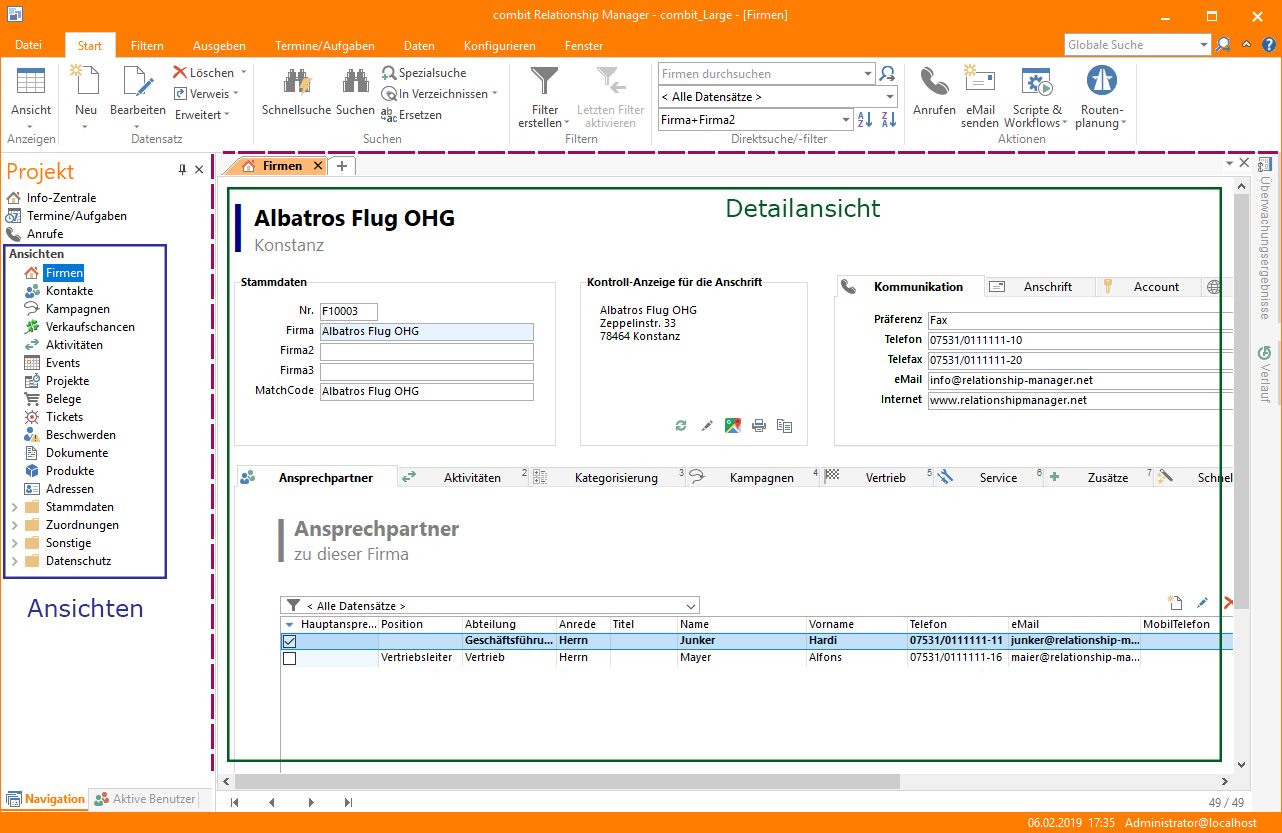
\includegraphics[width=\textwidth]{figures/crm_ui.png}
        \caption{Grafische Oberfläche des \gls{crm} Desktopclient (Februar 2019)}\label{fig:crm_ui}
\end{figure}

Aus technischer Sicht ist der \nameformat{\gls{crm}} in drei Schichten getrennt. Die zu verwaltenden Daten werden entweder in einer Microsoft SQL Server- oder einer PostgreSQL-Datenbank gespeichert. Eine Besonderheit hierbei ist die Tatsache, dass Relationen zwischen Datenbanktabellen nicht durch Fremdschlüssel und zugehörige Relationen auf Datenbankebene, sondern durch virtuelle Relationen zwischen einzelnen Ansichten im C++-Kern der Anwendung, realisiert sind. Dies erlaubt einen flexibleren Umgang mit diesen und vereinfacht das Ändern von Datenbanktabellen, Ansichten und Relationen direkt aus der Oberfläche des \nameformat{\gls{crm}}.
Der \nameformat{\gls{crm}}-Core bildet die zweite Schicht und ist für den Datenbankzugriff und die Business Logic\footnote{Anwendungslogik zwischen UI und Datenbank, welche programmspezifische (Verarbeitungs-) Regeln enthält} verantwortlich. Diese beiden Schichten sollen von der Erstellung der neuen Weboberfläche möglichst unberührt bleiben. Einzig die API-Anbindung für die UI muss an dieser Stelle integriert werden --- betrachtet wird die API in dieser Arbeit jedoch nur aus Sicht der Oberfläche, die Integration im Backend findet zu einem späteren Zeitpunkt statt.
Aufbauend auf dem Kern existieren parallel der Desktopclient, ebenfalls in C++ geschrieben, der WebAccess für Desktopbrowser und der WebAccess Mobile für mobile Endgeräte. Zwischen Core und Webaccess (Mobile) gibt es noch einen mit ASP.NET\footnote{Auf dem \.NET-Framework aufbauende Tools und Bibliotheken zum Erstellen von Web-Apps} realisierten .NET-Wrapper, welcher den Zugriff auf Daten per HTTP ermöglicht.

Abbildung~\ref{fig:crm_technical_stack} zeigt eine Übersicht der momentanen Architektur, Abbildung~\ref{fig:crm_future_technical_stack} hingegen, wie die Architektur in Zukunft aufgebaut sein könnte.

\begin{figure}
    \centering
    \captionsetup{justification=centering}
    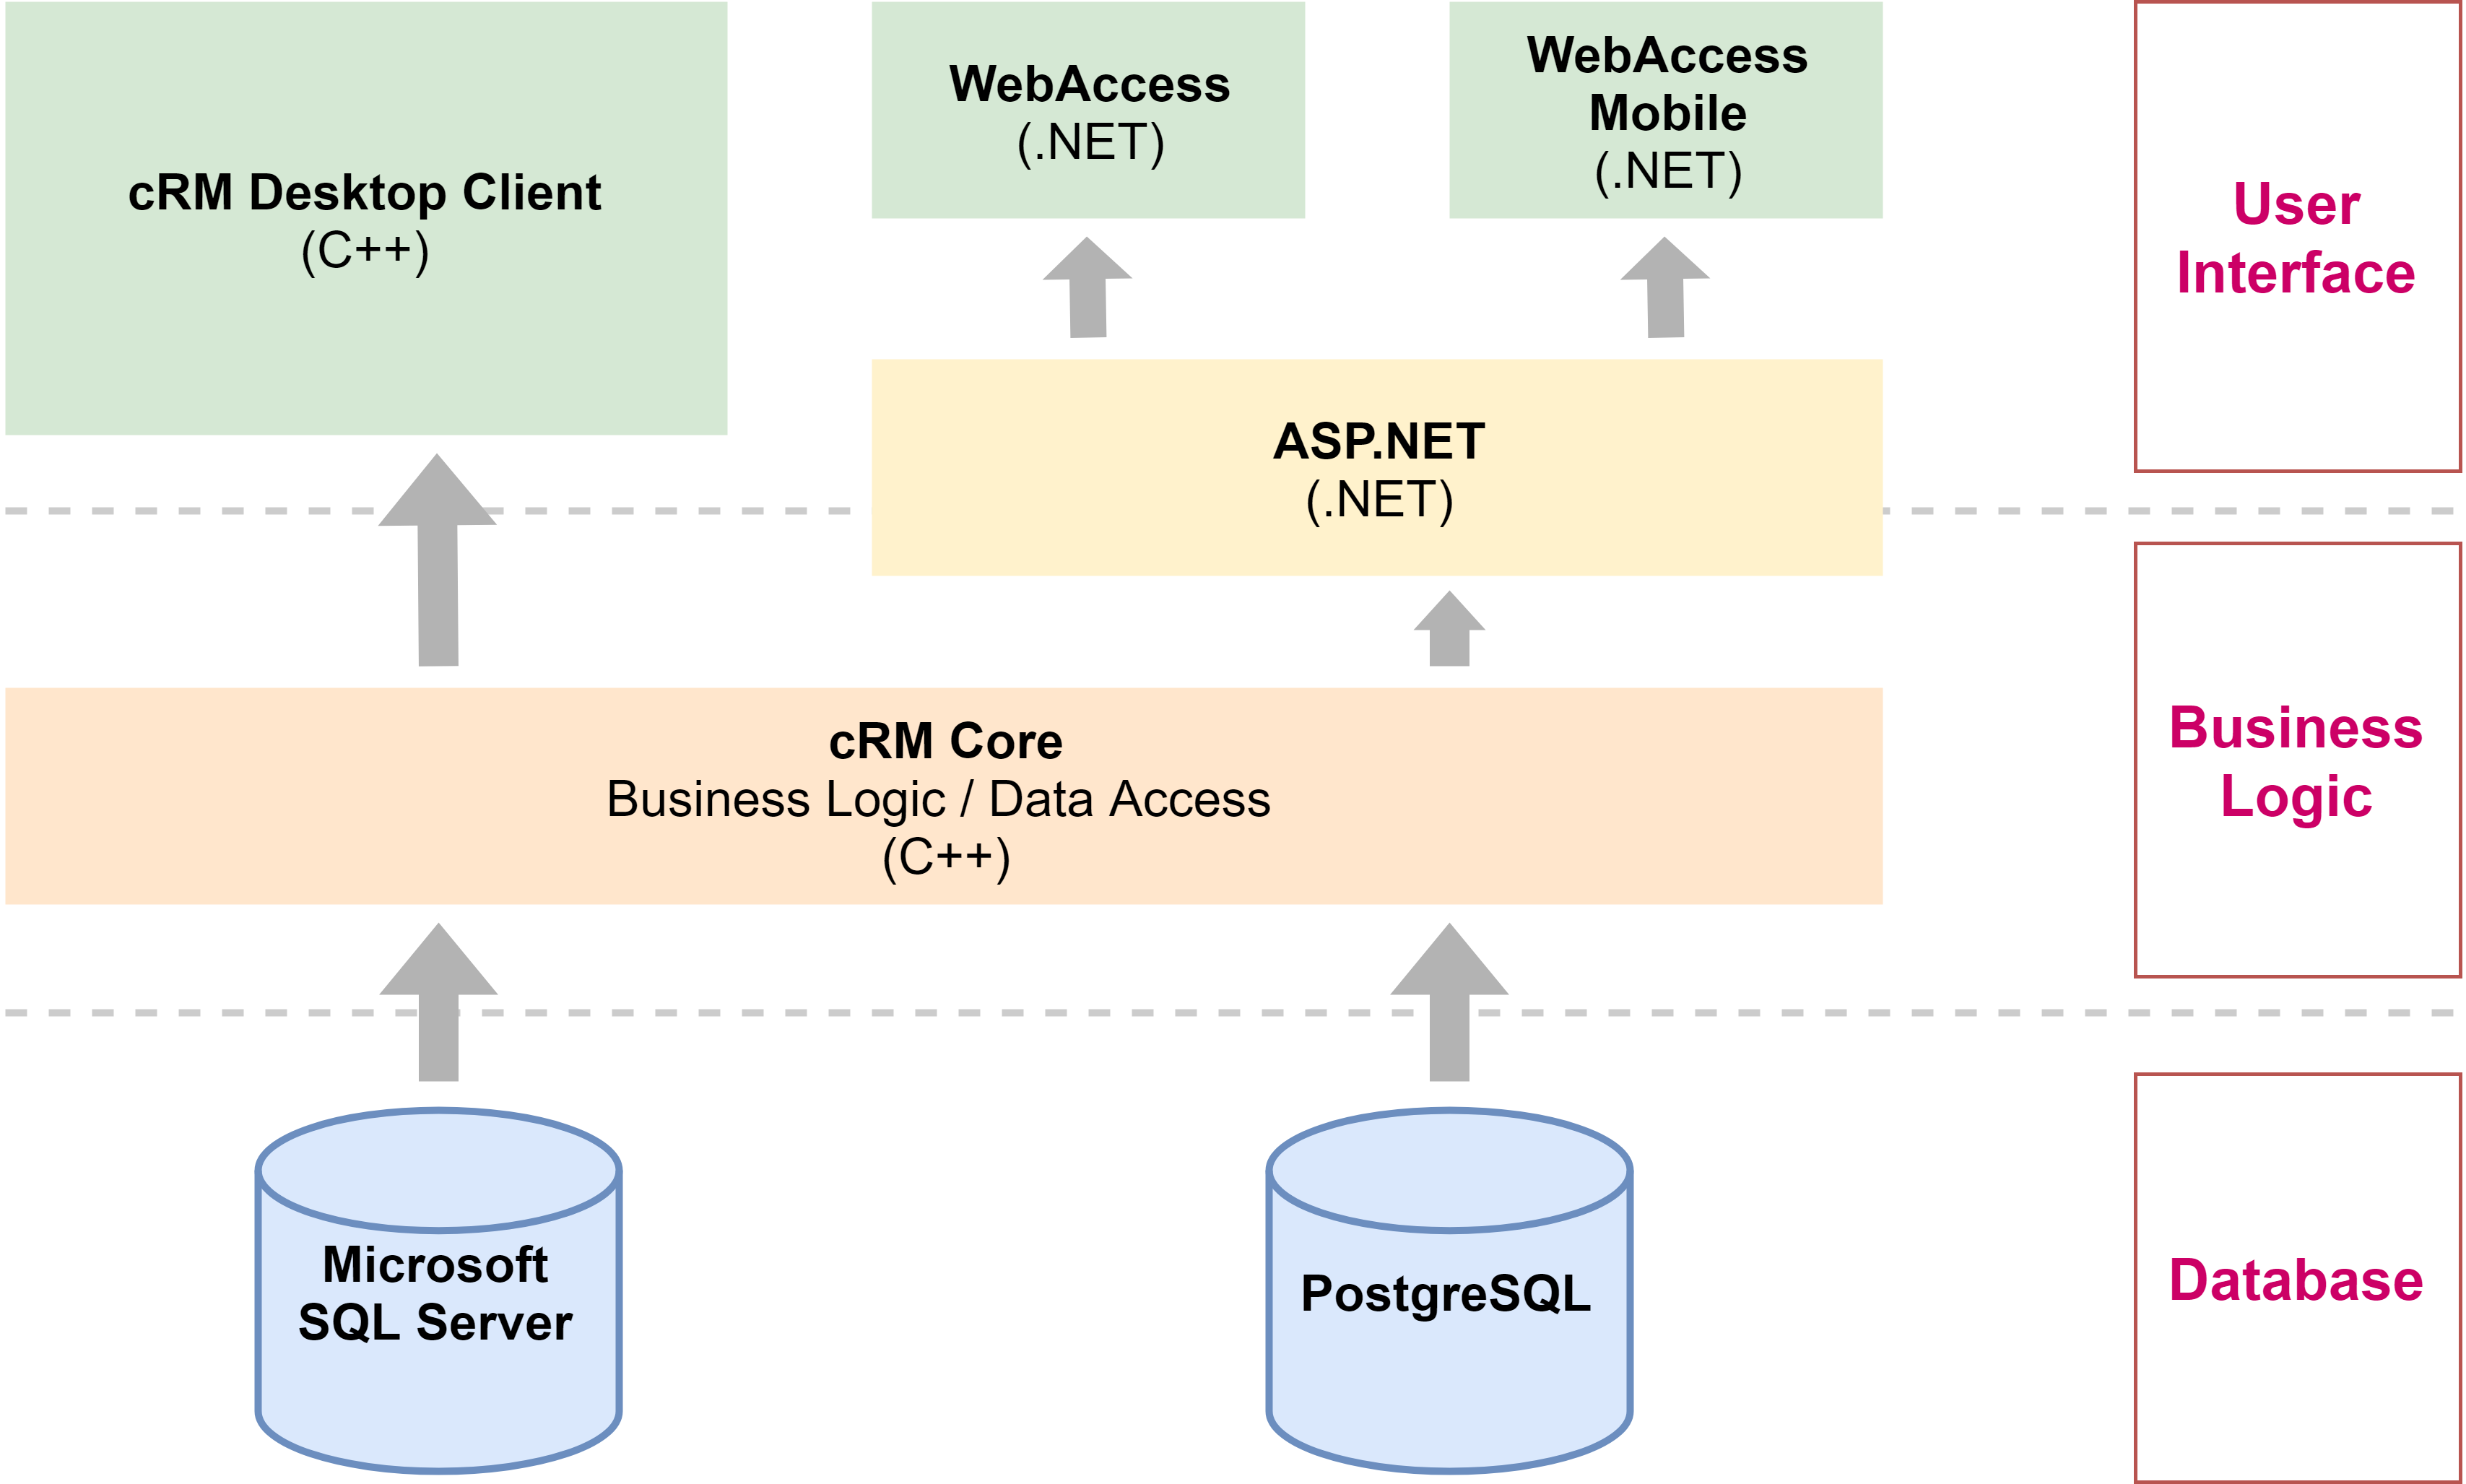
\includegraphics[width=\textwidth]{figures/crm_technical_stack.png}
        \caption{Aktueller technischer Aufbau des \gls{crm}}\label{fig:crm_technical_stack}
\end{figure}

\begin{figure}
    \centering
    \captionsetup{justification=centering}
    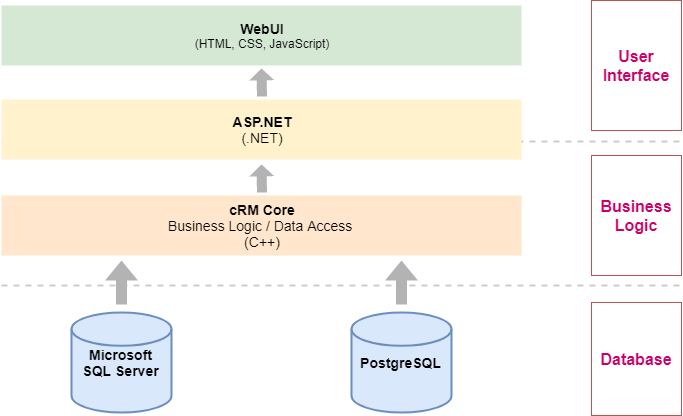
\includegraphics[width=\textwidth]{figures/crm_future_technical_stack.png}
        \caption{Möglicher, zukünftiger technischer Aufbau des \gls{crm}}\label{fig:crm_future_technical_stack}
\end{figure}


\section{Funktionale Anforderungen des \acrlong{crm}}
Dieser Teil des Kapitels befasst sich mit den funktionalen Anforderungen, welche sich direkt aus dem \gls{crm} und dessen bisherigen Eigenschaften und Funktionen ergeben.

\subsection{Automatisierte Erstellung der neuen UI}\label{subsec:func_req_automatic_ui_generation}
Die meisten Kunden haben entweder bereits ihre eigenen Ansichten erstellt oder benutzen angepasste Versionen der mitgelieferten Designs. Wird als langfristiges Ziel definiert, die komplette UI-Schicht ins Web zu überführen, muss das Ergebnis dieses Prozesses für die Benutzer leicht und zugänglich genug sein, um nicht schon im Voraus abgelehnt zu werden. Es ist daher essenziell, dass sämtliche bisherigen Ansichten mit minimalem Aufwand seitens der Nutzer im Web weiterverwendet werden können. Der minimale Aufwand meint dabei, dass im Ergebnis lediglich kleine Anpassungen tolerierbar sind, jedoch nicht die Neuerstellung jeder einzelnen Ansicht. Eines der Hauptziele dieser Arbeit ist es daher, eine automatische Umwandlung bestehender Ansichten zu ermöglichen. Hierfür muss die aktuelle UI-Spezifikation analysiert und eine neue Spezifikation erstellt werden, mithilfe derer Implementierungen aus den vorherigen abgeleitet werden können.

\subsection{Benutzerverwaltung}
Die Benutzer und deren Rechte werden vollständig im Backend verwaltet. Es muss allerdings bei der Umsetzung der Konfigurationsoberfläche und bei der Umsetzung der Rechte besonders sorgfältig geprüft werden, ob weiterhin der volle Funktionsumfang gewährleistet ist. Sollten bestimmte Rechte für Benutzer oder Gruppen nicht mehr anpassbar sein  oder fehlerhaft angewendet werden, ist unter Umständen der gesamte \nameformat{\gls{crm}} nicht mehr vernünftig nutzbar.

\subsection{Editier-Modus}\label{subsec:func_req_edit_mode}
Änderungen in der Detailansicht werden nicht direkt an die Datenbank übertragen, sondern nur als geändert markiert. Der Benutzer hat dann die Möglichkeit diese zu verwerfen oder den entsprechenden Datensatz zu speichern und die Informationen in die Datenbank zu schreiben.

\subsection{Individualisierung}\label{subsec:func_req_individualisation}
Die Individualisierung der beiden Hauptansichten für Datenentitäten, die Detail- und Listenansicht, ist zur effektiven Visualisierung bestimmter Sachverhalte ausschlaggebend. Bei der Listenansicht können beispielsweise Datenbankspalten ein- bzw.\ ausgeblendet und frei angeordnet werden, Spalten je nach Datentyp formatiert und spezielle Werte nach selbst definierten Regeln hervorgehoben werden. Die Detailansicht ist noch mächtiger, hier kann jedes UI-Element frei platziert werden, mit Sichtbarkeits- und Formatierungsbedingungen versehen und mit anderen Feldern verknüpft werden (verknüpft bedeutet: Änderung in Feld A löst Änderung in Feld B aus). Um diese Einstellungen vorzunehmen, ist ein Eingabemaskendesigner in die Software integriert, welcher dem Benutzer per \enquote{\gls{wysiwyg}}-Prinzip\footnote{Echtzeitdarstellung des Ergebnisses während der Erstellung und Bearbeitung} das Designen erleichtert.
Die Weboberfläche sollte diese Funktionalität möglichst vollständig abbilden.

\subsection{Berichts- und Webansicht}
Wie in Abschnitt~\ref{sec:product_overview} erwähnt, werden Berichte von einem zweiten Produkt der Firma \nameformat{combit GmbH}, dem sogenannten \nameformat{\gls{ll}}, gehandhabt. Dieses besitzt bereits zum jetzigen Zeitpunkt eine entsprechende Weboberfläche, die zukünftig für die Erstellung und das Anzeigen von Berichten genutzt werden kann. 
Auch die Webansicht kann weiterhin unterstützt werden, indem darin anzuzeigende Ressourcen in ein iframe-Tag\footnote{HTML-Element, welches das Einbetten von Dokumenten in andere Dokumente erlaubt} eingebunden werden.

\subsection{Suche / Filter / Sortierung}\label{subsec:func_req_search-filter-sorting}
Das Suchen und Filtern von Datensätzen kann weiterhin mit bestehenden Techniken gelöst werden, indem das Backend Daten vor dem Senden entsprechend im Vorfeld verarbeitet. Da es allerdings sinnvoll ist, Sortierungen in der Übersichtsliste auf dem Client auszuführen --- eine Garantie der API, dass Daten immer in einer entsprechenden Reihenfolge gesendet und auch empfangen werden, schränkt das Design dieser zu sehr ein --- ist es zumindest überlegenswert, ob das Suchen und Filtern ebenfalls zusätzlich direkt auf dem Client unterstützt werden soll. Viele JavaScript-Projekte bieten hierfür bereits fertige und effiziente Lösungen an, welche bei der Umsetzung genutzt werden können.

\subsection{Scripting}
Die Desktopanwendung des \nameformat{\gls{crm}} unterstützt momentan das Ausführen von Skripten in den Sprachen VBScript und C\#. Für die programmatische Ansteuerung existiert eine \gls{COM}-API, welche im Kontext des Clients, auf dem der Prozess ausgeführt wird, benutzt werden kann. Diese Technologien sind in einer Browserumgebung nicht verfügbar, daher kann ein Skript zwar über die neue UI ausgelöst, aber nicht lokal, sondern ausschließlich im Kontext des Servers ausgeführt werden. Existierende Skripte, welche darauf ausgelegt sind im Kontext des Clients ausgeführt zu werden, müssen vor der Nutzung in der Web-UI entsprechend angepasst werden.

\subsection{Import / Export}
Der Import und Export von Daten in und aus dem \nameformat{\gls{crm}} ist ein wichtiges Feature, wenn es darum geht, verschiedene Programme in einem Workflow zu vereinen. Der \nameformat{\gls{crm}} unterstützt diese Funktion mit einer Vielzahl an Formaten (Excel, Outlook, Datenbanken (ODBC) und Weitere). Diese Funktion kann, wie viele andere auch, weiterhin bestehen bleiben. Dafür muss jedoch eine Möglichkeit geschaffen werden, die Daten über das Netzwerk zur Verfügung zu stellen (Down- und Upload).

\subsection{Terminverwaltung und Aufgabenplanung}
Die interne Termin- und Aufgabenverwaltung ist analog zu anderen Daten über Datenbanktabellen realisiert. Diese können ebenso vom Backend an die Web-UI übertragen und dort dargestellt werden. Der Desktopclient unterstützt aber zudem auch die Verwaltung von Terminen von externen Programmen (z.B. \nameformat{Microsoft Outlook}). Eine Anbindung der neuen UI an diese kann nur gewährleistet werden, wenn entsprechende HTTP-APIs von den Produkten angeboten werden.

\subsection{Design für mobile und stationäre Endgeräte}
Da die neue Oberfläche alle bisherigen UI-Versionen ablösen soll, ist es ein zentrales Anliegen, sämtliche Endgeräte ihrer Möglichkeiten nach zu unterstützen. Eine bewährte Herangehensweise besteht darin, das mobile Design vor der Desktop-Ansicht zu gestalten. So können die wichtigsten Eigenschaften und Fähigkeiten des Designs direkt angelegt werden, während das Design für größere Bildschirme darauf aufbauend mit zusätzlichen Features, die speziell hierfür sinnvoll sind, ergänzt werden. Dieses Prinzip wird häufig \enquote{mobile-first}-Design genannt. Bei einer umgekehrten Vorgehensweise wird zuerst die Desktop-Ansicht mit allen verfügbaren Features und unter Ausnutzung des gesamten Bildschirmplatzes gestaltet. Dieses Design muss dann für mobile Geräte kompatibel gemacht werden, indem Features und Designelemente entfernt werden. Die Entscheidung, welche Aspekte dabei entfernt werden können, ist schwierig, da sie alle essenziell erscheinen.
Es ist zusätzlich auch wichtig zu beachten, dass viele mobile Nutzer --- je nach Standort --- keine ausreichend gute oder zumindest nur eine teilweise gute Internetverbindung besitzen und es daher wichtig ist, möglichst wenig Daten übertragen zu müssen, bevor eine Webseite angezeigt wird. Das für mobile Geräte charakteristische CSS sollte zuerst geladen werde, da dies weitere Downloads von irrelevanten Daten (CSS für nicht-mobile Geräte) vermeidet. Für stationäre Geräte ist eine derartige Optimierung jedoch nicht vonnöten.

\subsection{Vorerst nicht unterstützte Features}
Einige aktuelle Features des \gls{crm}s sind im Web entweder gar nicht oder nur mit sehr viel Aufwand umsetzbar. Diese werden daher vorerst nicht weiter beachtet und deren Umsetzbarkeit eventuell zu einem späteren Zeitpunkt erneut betrachtet:

\subsubsection{Scripting-Unterstützung auf dem Client}
Skripte werden momentan immer auf dem Client ausgeführt und evaluiert, dabei existiert u.a. Zugriff auf das Dateisystem und andere native Anbindungen des Betriebssystems. Da eine Webseite in der Browserumgebung aus Sicherheitsgründen vom restlichen Betriebssystem isoliert ist, können diese Möglichkeiten nicht genutzt und eine direkte Skriptausführung daher nicht unterstützt werden. 

\subsubsection{Interaktion mit anderen Prozessen}
 Bisher war es möglich, mit anderen Prozessen auf dem Client zu interagieren (Starten von externen Programmen, Interkation mit diesen per \gls{COM} etc.). Ein Beispiel hierfür ist ein Hilfsprogramm, mit dem Anrufe direkt am PC entgegengenommen und automatisch im \nameformat{\gls{crm}} protokolliert werden können. Eine derartige Interaktion ist in einer Browserumgebung, vor allem in einem, von fast allen gängigen Browsern benutzten Sandbox-Modus, nicht möglich.

\subsubsection{Ereignisse} 
Ereignisse sind Events, die zu bestimmten Zeitpunkten der Programmlaufzeit ausgelöst werden und als Aktion zum Beispiel ein Skript starten oder eine E-Mail versenden können. Bevor diese in der Web-UI implementiert werden können, muss zuerst evaluiert werden, welche dieser Ereignisse noch unterstützt werden können (Beispiel: Das Event \enquote{Nach Programmstart} --- anstatt eines Prozesses existiert nur noch eine Webseite. Das Laden dieser ist nicht gleichbedeutend mit dem Starten eines Prozesses, daher kann dieses Ereignis nicht mehr unterstützt werden.)

\section{Funktionale Anforderungen im Webbereich}
Zusätzlich zu den genannten Anforderungen gibt es im Web noch diejenigen Bereiche, die unterstützt werden sollten, um den Nutzern eine besonders gute Erfahrung bei der Bedienung der Seite zu ermöglichen, und solche Bereiche, die den Entwicklungsprozess positiv beeinflussen. Die wichtigstem dieser Anforderungen werden im Folgenden kurz erläutert. 

\subsection{i18n / l10n}
Die Akronyme \enquote{i18n} und \enquote{l10n} stehen für Internationalisierung respektive Lokalisierung \parencite{i18n_i10n_ishida_w3c_miller_boeing_2018}. Gemeint ist damit, dass für jede Sprachressource auf einer Webseite anstelle des Strings ein Identifikator genutzt wird, der mit Strings verschiedener Sprachen verknüpft ist. Je nach Einstellung (Auswahl durch Benutzer, Erkennung der Browsersprache etc.) können dann automatisch alle Texte in der jeweiligen Sprache angezeigt werden. Der \nameformat{\gls{crm}} unterstützt bereits mehrere Sprachen, die Ressourcen hierfür sind allerdings direkt in das Programm eingebettet. Um die gleiche Technologie für die Webseite nutzen zu können, müssten also sämtliche Texte durchweg aus dem Backend angefordert und über das Internet übertragen werden. Dies wäre nicht nur langsam und eine unnötige Belastung für den Server (Texte müssten bei jedem Aktualisieren der UI-Schicht neu geladen werden), sondern auch sehr fehleranfällig. Bei einer unterbrochenen Verbindung könnten überdies keine Fehlertexte angezeigt werden. Besonders im Hinblick auf den weiter unten beschriebenen \enquote{offline-first}-Ansatz sollten daher sämtliche Texte in der UI-Schicht gespeichert und jederzeit abrufbar sein.

\subsection{Barrierefreiheit}
Barrierefreiheit von Software bedeutet, dass diese auch von Menschen mit körperlichen Einschränkungen gut genutzt werden kann. Dies ist selbstverständlich immer ein wünschenswertes Ziel, zahlreiche Standards im Webbereich erleichtern ein solches Vorhaben jedoch in besonderem Maße. So gibt es beispielsweise bestimmte HTML-Tags, die extra dafür geschaffen wurden, um von Sprachsoftware vorgelesen zu werden. Weiterhin besteht die Möglichkeit per austauschbarem CSS einen \enquote{Dark Mode} anzubieten, sofern ein System von Beginn an entsprechend aufgebaut wurde.
Es sollte daher herausgearbeitet werden, welche Möglichkeiten für eine hohe Barrierefreiheit existieren und wie diese bei der Softwareentwicklung beachtet und umgesetzt werden können.

\subsection{Anleitungs-Modus / \enquote{Feature-Tour}}
 Um neuen Nutzern den Einstieg beim Erlernen eines Produkts zu erleichtern, kann ein interaktiver Anleitungs-Modus, welcher entweder beim ersten Aufruf einer Webseite und~/~oder bei der ersten Nutzung einzelner Features ausgelöst wird, hilfreich sein. Ein solcher Modus hebt wichtige Bedienelemente hervor und gibt kurze Erklärungen zu ebendiesen, welche entweder direkt durch einen Klick beendet werden können oder intelligent seltener erscheinen, je länger der jeweilige Nutzer das Produkt bereits kennt. Eine mögliche, fertige Umsetzung eines solchen Modus ist in Abbildung~\ref{fig:intro_js_example} von \nameformat{Intro.js} dargestellt.

 \begin{figure}
    \centering
    \captionsetup{justification=centering}
    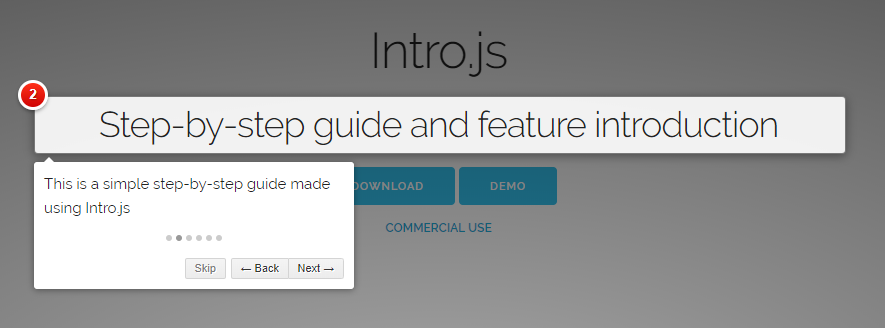
\includegraphics[width=\textwidth]{figures/intro_js_example.png}
        \caption{Anleitungs-Modus von Intro.js \parencite{mehrabani}}\label{fig:intro_js_example}
\end{figure}

\subsection{\enquote{Offline-First}-Ansatz}
In jüngster Zeit ist es möglich, mithilfe von Service-Workern\footnote{JavaScript-Proxy zwischen Webseite und Server; wird in einem anderen Thread als die eigentliche Webseite ausgeführt und kann Anfragen abfangen / verändern} und lokalen Speichermöglichkeiten im Browser Webseiten zu erstellen, die auch beim Aussetzen der Internetverbindung zumindest im Wesentlichen weiterhin funktionieren. So können etwa Änderungen, welche an den Server geschickt werden müssen, zwischengespeichert und, sobald wieder eine Verbindung zum Internet besteht, losgeschickt werden. Ein weiteres Beispiel ist das Anzeigen von Daten, die vom letzten Besuch einer Seite stammen, wenn beim aktuellen Aufruf die Verbindung nicht stabil genug ist. Natürlich sollte ein Nutzer über Änderungen des Status der Internetverbindung informiert werden.
Die Information über Verbindungsprobleme sowie die Antizipation ebendieser durch lokales Speichern von relevanten Informationen, zielen beide auf eine für mobile Nutzer möglichst komfortable Bedienung einer Webseite ab, was wie zuvor erwähnt, ein Hauptaugenmerk der neuen Oberfläche darstellt.

\subsection{Intelligente Fehlerbehandlung}
Softwarefehler auf eine für den Benutzer angenehme Art und Weise zu behandeln und im Nachhinein detailliert zu analysieren, ist bei traditioneller Software ein nicht zu unterschätzendes Problem. Bei Webapplikationen kommt jedoch erschwerend hinzu, dass ein Teil der Logik in einer Umgebung ausgeführt wird, welche durch herkömmliche Mittel nicht untersucht werden kann (Browser auf Clientrechner). Umso wichtiger ist es, ein Konzept zu entwickeln, welches in der entsprechenden Umgebung auftretende Fehler sowie Informationen zu deren Lösung übermittelt. Eine Option zur Lösung des Problems bestünde darin, auftretende Fehler immer direkt zum Server zu schicken, um sie vor Ort analysieren zu können. Wenn die eigene Infrastruktur dafür nicht ausreichend ausgebaut ist, gibt es auch entsprechende Online-Dienste, welche die Speicherung eines solchen Fehlerlogs ermöglichen. Zusätzlich dazu müssen auch Parameter für Serveranfragen mit höchster Vorsicht ausgewählt werden: Timeouts müssen lange genug sein, um eine Serverantwort nicht fälschlicherweise zu verwerfen und kurz genug, um bei einem tatsächlichen Fehler die Applikation nicht zu träge wirken zu lassen. Zudem sollten im Fehlerfall erneute Versuche intelligent gestartet werden, das heißt weder zu häufig noch zu selten, um den Server nicht unnötig zu belasten respektive um dennoch einen responsiven Eindruck zu vermitteln.

\subsection{Etablierte Authentifizierung}
Der \nameformat{\gls{crm}} besitzt zwar bereits ein integriertes Benutzersystem mit Authentifizierung und Rechteverwaltung, für die Portierung der Oberfläche sollte aber in Erwägung gezogen werden, diese Rechteverwaltung mit einem oft genutzten, öffentlichen Protokoll wie \nameformat{OAuth} oder ähnlichen Protokollen zu koppeln, um die Verbindung über HTTP und den Schutz der Authentisierungsdaten nicht mit einer selbst entwickelten, schlechter funktionierenden Lösung handhaben zu müssen.

\subsection{Caching}
Um Ressourcen zu sparen, ist es von Vorteil komplexe Berechnungen und zeitintensive Übertragungen nicht mehrmals, etwa bei mehrfachem Laden einer Webseite, auszuführen. Im Bereich des Webs gibt es mehrere Möglichkeiten solche Daten temporär zu speichern: Die einfachste Form besteht darin, Antworten auf eingehende Anfragen auf dem Server und ebenso danach auf dem Client wiederzuverwenden. Wenn der Client selbst kein Caching unterstützt, kann mit \enquote{bedingten Anfragen} dennoch der Cache des Servers genutzt werden: Es wird hierbei eine Anfrage an den Server geschickt und, sollte sich die Antwort im Vergleich zur letzten Anfrage nicht geändert haben, keine Daten, sondern nur ein entsprechender Hinweis an den Client zurückgesendet. Auch das HTTP-Protokoll unterstützt Mechanismen um Caching, beispielsweise über Cache-Proxies, zu erleichtern (spezielle Header, welche die Gültigkeitsdauer einer gespeicherten Ressource bestimmen). Bei allen Formen des Caching ist es jedoch kritisch, dass die richtige Strategie zum Invalidieren der Daten ausgewählt wird, um nicht mit veralteten Werten zu arbeiten, aber dennoch eine Effizienzsteigerung zu erreichen.

\subsection{Container}
Container-Technologien wie Docker und Kubernetes helfen dabei Abhängigkeiten der eigenen Software zu verwalten und auf jedem Entwicklungsrechner eine identische Umgebung zu schaffen. Auch für die Bereitstellung eines Service für Kunden ist es sehr viel einfacher einen bereits korrekt konfigurierten Container zu starten, anstatt eine vollständige Umgebung auf einem Server einzurichten. Dies gilt insbesondere wenn dieser Server von externen Dienstleistern verwaltet wird. Da diese Konzepte bei der \nameformat{combit GmbH} noch nicht eingesetzt werden, ist es sinnvoll zu untersuchen, an welchen Stellen diese zu mehr Produktivität in Entwicklung und Verteilung der Software beitragen könnten.

\subsection{Serverless}
Unter \enquote{Serverless} wird das Konzept verstanden, dass Firmen keine eigenen Server für ihre Kunden oder eigene Zwecke einrichten müssen, sondern auf Lösungen von Drittherstellern (etwa \nameformat{AWS} von \nameformat{Amazon} oder \nameformat{Microsoft Azure}) zurückgreifen können, auf welchen die eigene Software ausgeführt wird. Firmenintern wird also kein Server betrieben, die eigene Infrastruktur ist demnach \enquote{Serverless}. Der Vorteil dieses Ansatzes ist, dass die Verantwortung über die Serverhardware nicht selbst getragen werden muss und die Server durch die großen Kapazitäten der Hersteller je nach Belastung skaliert werden können. Im Gegenzug werden aber eigene Daten fremden Servern anvertraut, je nach Art und Sensibilität der Daten (Betriebsgeheimnisse, \gls{dsgvo}) kann dies nicht gewünscht sein. Ein solcher Ansatz muss daher gut abgewogen werden, bevor er weiter verfolgt werden kann.

\subsection{Aktualisierungsstrategie}
Kontinuierliche Softwareupdates zur Fehlerverbesserung oder zur Ergänzung neuer Features zählen heutzutage zum Standardservice. Wenn dieser Service angeboten werden soll bedarf es einer kompetenten Strategie, um Modifikationen und Erweiterungen an die Nutzer auszuliefern. Das Backend, auf dem auch die UI-Schicht gehostet werden soll, wird von den Kunden betrieben. Es unterliegt damit nicht dem Verwaltungsbereich der \nameformat{combit GmbH}, weshalb Updates nicht direkt dort eingespielt werden können. Anstatt Updates für die Oberfläche an Updates des Backends zu koppeln, sollte überlegt werden, ob eine konfigurierbare Option angeboten werden kann, durch die Updateprüfungen auf einem zentralen \nameformat{combit}-Server ausgeführt werden. Dies setzt allerdings voraus, dass verschiedene Versionen der Oberfläche und des Backend miteinander kompatibel sind. 

\subsection{Integration von bestehenden Ressourcen}
Auf der Webseite der \nameformat{combit GmbH} gibt es bereits zahlreiche Ressourcen wie FAQ oder eine Knowledgebase zu verschiedenen Produkten. Um Nutzern diese Ressourcen präsent zu machen, könnten diese direkt in die Oberfläche, etwa im Rahmen eines Hilfe-Modus, integriert werden.

\section{Anforderungen an den Entwicklungsprozess}
Neben den funktionalen Anforderungen ist es ebenso wichtig, die richtigen Anforderungen für die Projektumgebung und -entwicklung zu formulieren, um diesen Prozess möglichst effizient und skalierbar zu halten. Daher wird empfohlen, folgende Technologien und Praktiken bei der Entwicklung des neuen Projektes zu nutzen:

\subsection{Tests}
Alle in Kapitel~\ref{chap:technologies} vorgestellten UI-Frameworks enthalten bereits Lösungen zur Ausführung von Tests. Eine hohe Testabdeckung ist daher nicht nur nützlich, um die Codequalität zu erhalten und Regressionen zu erkennen, sondern auch ohne hohe Kosten und Aufwand erreichbar.

\subsection{Continuous Integration}
Ein für diesen Zweck geeigneter \nameformat{TeamCity}-Server von der Firma \nameformat{JetBrains} ist firmenintern bereits vorhanden, daher sollten Tests von neuen Features immer auch auf diesem Server ausgeführt werden.

\subsection{Codereviews}
Pro Feature sollte auf einem gesonderten Branch gearbeitet und beim Zurückführen in den Masterbranch ein Review durch mindestens einen anderen Entwickler stattfinden, um die Codequalität stets auf einem hohen Niveau zu halten. Auch für Reviews gibt es firmenintern bereits einen \nameformat{Upsource}-Server (ebenfalls von der Firma \nameformat{JetBrains}), welcher mit dem \nameformat{TeamCity}-Server zusammen genutzt werden kann.

\section{Hauptaugenmerk dieser Arbeit}
Eine komplette Umsetzung aller Anforderungen wäre im Rahmen dieser Thesis nicht zu bewältigen. Es gäbe zu viele Aspekte (geeignetes Hosting, eine sichere Authentifizierungsmethode, ein neuer Aktualisierungsmechanismus etc.), die beachtet werden müssen. Summiert reicht die Zeit nicht aus, um Konzepte für all diese Aspekte in einer entsprechenden Qualität und Sorgfalt zu erstellen und umzusetzen. 
Wie in diesem Kapitel bereits beschrieben, kann die Oberfläche des \nameformat{\gls{crm}} in zwei Hauptbereiche unterteilt werden. Zum einen existieren diejenigen UI-Bereiche, welche sich nicht mit den anzuzeigenden Daten ändern, wie in Abbildung~\ref{fig:crm_ui} links und oberhalb der Detailansicht erkennbar wird (weitere Dialoge und Oberflächen werden kontextbasiert angezeigt), und zum anderen die Detail- und Listenansicht selbst. Die nicht datenabhängigen Elemente und Dialoge bestehen fast vollständig aus statischen Elementen mit teilweise speziellen Anforderungen, welche bei der Umsetzung zwar zeitaufwändig wären, technisch jedoch kein interessantes Problem darstellten. Es werden im Weiteren daher nur die Oberfläche der Datenansichten (Detail- und Listenansicht) und die damit verbundenen Anforderungen betrachtet.
Aus der Liste der funktionalen Anforderungen des \nameformat{\gls{crm}} werden also insbesondere die Automatisierte Erstellung~\ref{subsec:func_req_automatic_ui_generation}, der Editier-Modus~\ref{subsec:func_req_edit_mode}, die Individualisierung~\ref{subsec:func_req_individualisation} und die Unterstützung der Suche, Filter und Sortierungen~\ref{subsec:func_req_individualisation} beachtet.

Ein Vorteil von moderner, komponentenbasierter Webtechnologie (alle in Kapitel~\ref{chap:technologies} betrachteten Frameworks sind darauf ausgelegt) ist es, trotz der getrennten Entwicklung verschiedener UI-Bestandteile diese problemlos miteinander zu kombinieren zu können. Es ist sogar möglich unterschiedliche Technologien für die jeweiligen Teile zu nutzen, da zur Laufzeit alle Framework-Umsetzungen in herkömmliches JavaScript, HTML und CSS transpiliert\footnote{Übersetzung von Quellcode aus einer Programmiersprache in eine andere} werden und somit miteinander kompatibel sind.
Bei dieser zweistufigen Umsetzung kann das Ergebnis dieser Arbeit außerdem bereits in der Webansicht der bestehenden Desktopapplikation angezeigt und als Alternative zu den nativen Oberflächen angeboten werden. So können Kunden dieses Feature bei Interesse bereits im Vorfeld testen, evaluieren und wichtiges Feedback für die weitere Entwicklung einbringen.

\chapter{Technologien}\label{chap:technologies}

Die richtige Technologie zur Lösung einer Problemstellung auszuwählen garantiert noch keinen Erfolg, ist aber ein wichtiger Grundstein um überhaupt erfolgreich sein zu können. In diesem Sinne sollte nicht zu wenig Augenmerk auf den Vergleich und die Entscheidung zwischen auf dem Markt verfügbaren Alternativen gelegt werden. Dieses Kapitel beschreibt, welche Technologien für welchen Teil der Architektur in Frage kommen, stellt diese gegenüber und begründet die Entscheidung für die am besten geeignetste Alternative.

\section{Entwicklungsumgebung}
Die Entwicklung des \nameformat{\gls{crm}} findet momentan ausschließlich mit \nameformat{Microsoft Visual Studio} statt. Wie in Kapitel~\ref{chap:requirements} ist gibt es die Core-Komponente und Desktopkomponente, welche in C++ geschrieben sind, und eine auf den Core aufsetzende, in C\# geschrieben, .NET-Komponente zur Bereitstellung der Webfunktionalität. Der bestehende Entwicklungsprozess soll nicht verändert und auch nicht weiter thematisiert werden, da die neu zu entwickelnde UI-Schicht eine unabhängige Codebasis besitzt und auch konzeptionell von den bisherigen Schichten getrennt ist. 

Für das in Kapitel~\ref{chap:requirements} angesprochene Tool zum Einlesen und Konvertieren der bisherigen UI-Repräsentation wurde wegen der vorhandenen internen Infrastruktur ebenfalls Visual Studio verwendet. Die Wahl der Programmiersprache fiel auf C\#, da der Zugriff auf das Dateisystem und speziell auf XML-Dateien, das Format der momentanen Repräsentation, sehr einfach ist. 

Für die neu entstehenden Webtechnologien kann jeder beliebige Texteditor benutzt werden, da keine speziellen Funktionen einer IDE oder eines Editors notwendig sind. Der in den nachfolgenden Kapiteln entwickelte Code wurde aufgrund der guten Autovervollständigung, der Integration mit Versionsverwaltungstools und der einfachen Erweiterbarkeit, mit \nameformat{Visual Studio Code} von \nameformat{Microsoft} erstellt. Wichtiger als der Editor ist die Sprache für welche er benutzt wird. Im Bereich der Webentwicklung hat sich JavaScript ohne Konkurrenz durchgesetzt und ist die einzige Sprache, die von allen Browsern unterstützt wird. Das spiegelt sich auch in der Auswahl der Frontend-Frameworks wieder, welche alle entweder direkt oder indirekt in JavaScript geschrieben sind.   

\section{Frontend-Frameworks}
\subsection{Traditionelle Lösungen}
Frameworks und Bibliotheken die versuchen Entwicklern das Erstellen von UIs zu erleichtern gibt es schon sehr lange und in einer sehr großen Anzahl. Traditionelle Projekte wie jQuery-UI (Mobile), Bootstrap und neuere Namen (Materialize, Semantic-UI, Pure, etc.) setzen auf die Gestaltung von fertigen Komponenten die per CSS-Klasse in eine vorhandene Webseite integriert werden können. Durch diesen Fokus auf pures Styling mit CSS sind diese Projekte meist sehr klein und können schnell integriert werden. Sie eignen sich damit für rapides Prototyping, jedoch nicht um komplette Webseiten von Grund auf zu erstellen --- vielmehr können sie mit den unten angesprochenen JavaScript-Projekten im Zusammenspiel benutzt werden.

\subsection{Moderne, JavaScript-basierte Lösungen}
In diesem Bereich sind vor allem komponentenbasierte Frameworks basierend auf einem virtuellen DOM\footnote{Virtuelle und meist vereinfachte Repräsentation der UI im Speicher, wird Framework-intern mit dem echten DOM synchronisiert} stark verbreitet. Aufgrund der zeitlichen Limitierung dieser Arbeit ist es nicht möglich die große Auswahl an Alternativen zu betrachtet. Es werden daher nur die drei größten Mitstreiter \nameformat{Vue}, \nameformat{React} und \nameformat{Angular} \parencite{greif_benitte_rambeau_2018} miteinander verglichen. Weitere Möglichkeiten für spätere Analysen sind \nameformat{Polymer}, \nameformat{Ember}, \nameformat{Knockout}, \nameformat{Riot}, etc.

\subsection{Vergleich Vue, React \& Angular}

\subsubsection{Generell}
\begin{itemize}
    \item{Vue}
    \item[] Entwickler legen viel Wert darauf möglichst kleine und dennoch performante Laufzeit zu entwickeln. Der Einstieg in \nameformat{Vue} soll möglichst einfach sein, was durch eine sehr gute Dokumentation und ein hervorragendes \gls{cli}-Tool\footnote{Kommandozeilen-Oberfläche} zum Erstellen neuer Projekte gelingt. Abhängigkeiten zwischen Daten und UI verfolgt Vue selbstständig, es werden daher immer nur Elemente aktualisiert wenn sich auch deren anzuzeigende Daten geändert haben. Das Erstellen von nativen Apps ist bei \nameformat{Vue} nur mit Software von Drittherstellern möglich, die Entwickler arbeiten mit diesen aber zusammen um den Prozess zu verbessern. Das Verwenden von JavaScript-Templates (JSX) und \nameformat{Typescript} ist mit etwas Konfiguration ebenfalls möglich. \nameformat{Vue} hat im Vergleich noch ein kleines Ökosystem, kann aber dafür den stärksten Wachstum aller Frameworks verzeichnen.
    \item{React}
    \item[] \nameformat{React} diktiert im Vergleich zu \nameformat{Vue} noch weniger Vorgaben an die Entwickler, alle typischen Problemstellungen werden durch Bibliotheken gelöst. Dies ist möglich, da das Ökosystem sehr groß ist und eine breite und tiefe Auswahl an entsprechenden Bibliotheken bietet. Native Apps können mit dem vom gleichen Team entwickelten \nameformat{React-Native} erstellt werden ohne dafür weitere Software zu benötigen. Durch die Konzentration auf wesentliche Features und Verbesserungen und eine stabile API stellt das \nameformat{React}-Team sicher, dass Upgrades auf neue Versionen gar keine bis wenige Änderungen am bestehenden Code verlangen. Auch \nameformat{Typescript}-Integration und damit verbundenes Tooling (Linter, Type checks, Autocompletion) sind problemlos möglich.
    \item{Angular}
    \item[] Es werden für alle typischen Anforderungen die bei der Entwicklung anfallen bereits Tools und Konzepte mit ausgeliefert, um diese Anforderungen zu erfüllen. Dadurch ist \nameformat{Angular} an sich sehr viel mächtiger als \nameformat{Vue} und \nameformat{React}. Die Chance dafür dass man abgesehen von \nameformat{Angular} noch weitere große Bibliotheken benötigt ist gering, jedoch erfordert die Nutzung dieser mitgelieferten Möglichkeiten auch dass man sie gut genug kennt. Der Einstieg in \nameformat{Angular} wird von vielen daher als mühsam und zeitintensiv beschrieben. Die Dokumentation ist sehr umfangreich, teilweise aber auch unübersichtlich und das Ökosystem von \nameformat{Angular} ist zwar größer als das von \nameformat{Vue}, es hat jedoch auch negatives Wachstum zu verzeichnen.
\end{itemize}

\subsubsection{Aufbau von Apps (mit Beispielkomponente)}
Um zumindest ein Gefühl für das Benutzen der jeweiligen Frameworks zu bekommen wurde eine Beispielkomponente ausgewählt die mit allen drei Frameworks umgesetzt werden soll. In Abbildung~\ref{fig:example_component} sieht man die fertige Komponente. Bei Klick in das Edit-Feld ändert sich die Farbe des Randes um den Fokus zu signalisieren. Ändert man den Eintrag kann diese Änderung mit Escape verworfen oder mit Enter gespeichert werden. Der Text darunter gibt immer den momentan gespeicherten Wert wieder. Die Komponente wurde in Online-Editoren erstellt welche bereits eine fertig Umgebung mit dem jeweiligen Framework bieten. Auf die Benutzung weiterer Bibliotheken wurde hier explizit verzichtet.

\begin{figure}
    \centering
    \captionsetup{justification=centering}
    
\includegraphics{figures/example_component.png}
        \caption{Beispielkomponente für die Umsetzung mit allen Frameworks}\label{fig:example_component}
\end{figure}


\begin{itemize}
    \captionsetup{justification=centering}
    \item{Vue}
    \item[] Die \nameformat{Vue}-Komponente wird komplett als Instanz einer \nameformat{Vue}-Klasse angelegt, der man Daten und Methoden übergeben muss. Im HTML-Template werden die \nameformat{Vue}-eigenen Attribute ersichtlich.
    \item[] \lstinputlisting[language={JavaScript}, label={lst:vue_example},caption={Umsetzung der Beispielkomponente mit Vue}]{code/chapter_003_vue_example.js}
    \item{React}
    \item[] Eine \nameformat{React}-Komponente kann entweder als herkömmliche Klasse oder nur als Funktion, welche die darzustellenden UI-Elemente als Rückgabewert enthält, angegeben werden.
    \item[] \lstinputlisting[language={JavaScript}, label={lst:react_example},caption={Umsetzung der Beispielkomponente mit React}]{code/chapter_003_react_example.js}
    \item[] \lstinputlisting[language={JavaScript}, label={lst:react_hooks_example},caption={Funktionale Umsetzung der Beispielkomponente mit React}]{code/chapter_003_react_hooks_example.js}
    \item{Angular}
    \item[] Bei \nameformat{Angular} besteht eine Komponente wie bei \nameformat{React} aus einer herkömmlichen Klasse. Diese wird jedoch mit einer speziellen Annotation mit Informationen über das Aussehen und die Platzierung der Komponente versehen.
    \item[] \lstinputlisting[language={JavaScript}, label={lst:angular_example},caption={Umsetzung der Beispielkomponente mit Angular}]{code/chapter_003_angular_example.js}
\end{itemize}

\subsubsection{State-Management}
\begin{itemize}
    \item{Vue}
    \item[] Standard ist, dass jede Komponente ihr eigenes State-Objekt besitzt. Zusätzlich dazu kann noch auf das State-Objekt der \nameformat{Vue}-Instanz in der sich die Komponente befindet (Parent) zugegriffen werden. Dieses kann entweder direkt verändert oder per Store-Pattern\footnote{Geteilter State wird zentral verwaltet, Änderungen am State nur intern möglich} verwaltet werden. \nameformat{Vuex} ist eine direkt von \nameformat{Vue} entwickelte Bibliothek welche das genannte Store-Pattern umsetzt.
    \item{React}
    \item[] \nameformat{React} unterstützt nur einen unidirektionalen Datenfluss mit ``Props''. Diese werden Komponenten von ihren Elternkomponenten mitgegeben. Jede Komponente hat ihren eigenen State der per Props an Kinder weitergegeben (aber nicht direkt verändert) werden kann. Es gibt einige bekannte Bibliotheken welche das Verwaltung von State auf andere Arten lösen. \nameformat{Redux} setzt das funktionale Flux-Pattern um, dabei werden Änderungen per Aktions-Event ausgelöst, die Events von Reducern ausgewertet und der State entsprechend verändert. Der neue State wird den entsprechenden UI-Elementen wieder unveränderbar (immutable) übergeben. \nameformat{MobX} und \nameformat{react-easy-state} setzen das bei \nameformat{Vue} erwähnte Store-Pattern in \nameformat{React} um.
    \item{Angular}
    \item[] State wird direkt in den Klasseninstanzen der Komponenten gespeichert und kann durch herkömmliche Konzepte der objektorientierten Programmierung weitergegeben und verändert werden. Zusätzlich existiert auch \nameformat{NGXS}, welches auf dem gleichen Prinzip wie \nameformat{Redux} beruht, aufgrund moderner \nameformat{Typescript}-Features laut \nameformat{Angular} aber einfacher zu benutzen sei.
\end{itemize}

\subsubsection{Routing}
\begin{itemize}
    \item{Vue}
    \item[] Routing ist direkt in \nameformat{Vue} integriert. Routen werden in JavaScript mit Komponenten verknüpft und bei Aufruf dieser Route wird die verknüpfte Komponente an einen zuvor festgelegten Platzhalter im DOM gerendert.
    \item{React}
    \item[] Nicht integriert, es gibt aber mehrere Alternativen als Bibliotheken. Bei \nameformat{Aviator} werden Routen als geschachteltes Objekt übergeben, bei dem jedes Element eine Route und eine Zielfunktion enthält. Die Zielfunktion wird aufgerufen wenn zur entsprechenden Route navigiert wird und muss wissen wie und wohin (etwa über Dokument-Selektoren) die entsprechende Komponente gerendert werden muss. Die Nutzung von JSX ist dabei nicht mehr möglich. Bei \nameformat{react-router} hingegen werden die Routen deklarativ in den JSX-Templates hinterlegt. Sie enthalten als Property die Route für die sie gerendert werden sollen und die eigentliche Komponente die angezeigt werden soll.
    \item{Angular}
    \item[] Analog zu \nameformat{Vue} ist auch hier eine Lösung direkt integriert und funktioniert auch nach dem exakt gleichen Prinzip.
\end{itemize}

\subsubsection{Testing}
\begin{itemize}
    \item{Vue}
    \item[] \nameformat{Vue} enthält Test-Tools mit denen man Komponenten in Variablen rendern kann. Diese gespeicherten Komponenten sind herkömmliche JavaScript-Objekte und können dann mit weiteren (externen) Tools auf bestimmte Zustände und Eigenschaften geprüft werden.
    \item{React}
    \item[] Das Testen von \nameformat{React}-Komponenten funktioniert analog zu \nameformat{Vue}.
    \item{Angular}
    \item[] Alle zum Testen benötigten Tools sind bereits enthalten und sehr ausführlich dokumentiert. Wenn nur bestimmte Teilaspekte einer Anwendung wie etwa die UI-Komponenten getestet werden sollen ist der Aufwand dies einzurichten durch die Notwendigkeit sich mit dem kompletten Test-Konzept auseinander setzen zu müssen höher als bei \nameformat{Vue} und \nameformat{React}.
\end{itemize}

\subsubsection{\acrlong{ssr}}
Bei allen Frameworks gibt es auch die Möglichkeit nur wenige Seiten ``vor-gerendert'' auf dem Server liegen zu haben anstatt sie dynamisch bei entsprechenden Anfragen zu generieren. Hierfür kann das \nameformat{Node.js} Tool \nameformat{Prerender.io} benutzt werden.
\begin{itemize}
    \item{Vue}
    \item[] \nameformat{Vue} liefert einen dafür vorgesehenen Renderer (\nameformat{vue-server-renderer}) der Markup als Text generiert. Das kann beim initialen Laden der Seite ausgeliefert werden (erfordert einen \nameformat{Node.js} Server).
    \item{React}
    \item[] Auch \nameformat{React} liefert einen dafür vorgesehenen Renderer (\nameformat{ReactDOMServer}) der Markup als Text generiert. Das kann beim initialen Laden der Seite ausgeliefert und auf Clientseite mit ReactDom.hydrate() mit Inhalten gefüllt werden (erfordert einen \nameformat{Node.js} Server).
    \item{Angular}
    \item[] \nameformat{Angular} benötigt für \gls{ssr} zusätzliche Abhängigkeiten, Änderungen an der Konfiguration, ein zusätzliches Build / Bundle Target und ein zusätzliches Modul mit extra Konfiguration das auf dem Server läuft und dafür zuständig ist das neue JS-Bundle auszuliefern.
\end{itemize}

\subsection{Fazit}
Alle betrachteten Alternativen sind valide Optionen mit denen jegliche Anforderungen umgesetzt werden können. Der Einstieg in \nameformat{Angular} scheint allerdings schwierig, da dort eine Vielzahl an Technologien für verschiedenste Zwecke mitgeliefert werden. Da es seitens der Funktionalität kein Unterschiede gibt kommt es mehr oder weniger darauf an welches Projekt einem Entwickler (-team) am meisten zusagt bzw.\ mit welchem es am besten arbeiten kann.
\nameformat{React} besitzt mit Abstand die größte Community, es kann daher davon ausgegangen werden, dass die Weiterentwicklung, viele aufsetzende Bibliotheken und Ressourcen im Netz garantiert sind. Ein weiterer Vorteil, die Benutzung von \nameformat{Typescript} vorausgesetzt, ist die IDE-Unterstützung beim Schreiben der Komponenten-Templates. Im Vergleich zu \nameformat{Vue} wird bei \nameformat{React} hier ausschließlich JavaScript genutzt, was es erlaubt die Typisierung von \nameformat{Typescript} zu nutzen um Autovervollständigung oder ähnliche Hilfen anzuwenden. \nameformat{Vue} hingegen schreibt JavaScript-Funktionsaufrufe in Strings und nutzt eigene, für nicht \nameformat{Vue}-Entwickler unbekannte, HTML-Attribute für Schleifen und Verzweigungen --- da es sich dabei um \nameformat{Vue}-Sonderfälle handelt kann die IDE oft nicht helfen, es liegt also am Entwickler das entsprechende Wissen aufzubauen und keine Fehler zu machen.

Für den Prototypen wird vorerst \nameformat{React} genutzt. Da die die Technologien zur Laufzeit alle kompatibel sind (sie werden alle in normales HTML, CSS und JavaScript transpiliert), kann dieser Code später aber auch mit Vue zusammen genutzt oder nach und nach ersetzt werden.

\section{TypeScript}
Bei JavaScript handelt es sich um eine dynamisch typisierte Sprache, dass heißt das sich Typen von Variablen zur Laufzeit ändern können und vor der Nutzung einer Variablen entsprechend überprüft werden müssen. Dies ist ein Vorteil wenn schnell kleinere Skripte geschrieben werden bei denen aufgrund ihrer überschaubaren Größe entsprechende Überprüfungen trivial sind oder es schlichtweg keine Rolle spielt ob ein Skript Fehler enthält. Für die Entwicklung von größeren Projekten ist diese Eigenschaft jedoch ein gravierender Nachteil, da Typen von Variablen im Code durch Entfernung von Deklaration und Nutzung nicht ersichtlich sind und daraus resultierende Fehler bei der Benutzung immer erst zur Laufzeit der betroffenen Zeilen auftreten oder sogar gar nicht als Fehler erkennbar sind und lediglich ein falsches (aber nicht unbedingt als falsch erkennbares) Ergebnis liefern.   

Um dieser Art von subtilen Bugs vorzubeugen bietet \nameformat{Microsoft} seit 2012 \nameformat{TypeScript} an. Es handelt sich dabei um eine typisierte open-source Sprache welche als syntaktische Obermenge von JavaScript (normaler JavaScript-Code ist also ebenso gültiger \nameformat{TypeScript}-Code) beschrieben werden kann und die zu gewöhnlichem JavaScript transpiliert\footnote{Übersetzung von Quellcode aus einer Programmiersprache in eine andere} wird und somit trotz ihrer Vorteile keinen Kompatibilitätsnachteil besitzt. Da die Syntax auf JavaScript basiert ist das Erlernen dieser für JavaScript-Entwickler trivial. Durch Nutzung von typisierten Daten werden fehlerhafte Nutzungen von Variablen bereits bei der Entwicklung, eine entsprechende Integration des Editors vorausgesetzt, oder spätestens beim Transpilieren bemerkt und dem Entwickler als solche angezeigt. Ebenso erlaubt eine Editorintegration das Anbieten von Codevervollständigung und damit zu einem effektiveren Entwicklungsprozess.

Der einzige Nachteil von \nameformat{TypeScript} ist, dass ein zusätzlicher Schritt zum Übersetzen in JavaScript-Code notwendig ist. Da die meisten Projekte im Webbereich aber sowieso nicht komplett ohne ähnliche Tooling-Schritte auskommen und der \nameformat{TypeScript}-Compiler einfach in diese bestehenden Prozesse integrierbar ist handelt es sich hierbei nur um eine überschaubare Einschränkung. Dieser Nachteil kann aber auch positiv ausgelegt werden, da es durch den Übersetzungsschritt möglich ist, bereits Features und Standards zu benutzen, welche noch nicht von allen Browsern unterstützt werden. Bei der Übersetzung werden diese in semantisch identischen Code umgewandelt, der unter Einhaltung von älteren Standards gültig ist, aber für den Entwickler schwieriger zu schreiben wäre. 

Aufgrund dieser Argumentation soll zur Unterstützung der Entwickler und Vorbeugen von Fehlern bei die Entwicklung der \nameformat{React}-Seite ausschließlich \nameformat{TypeScript} benutzt werden. 

\section{API-Anbindung}
Die Anbindung der API kommen zwei Ansätze in Frage: \nameformat{Rest} und \nameformat{GraphQL}\@. Bei \nameformat{Rest} handelt es sich um einen Architekturstil bei dem Ressourcen über URI-Endpunkte angesprochen und abgerufen werden. \nameformat{GraphQL} hingegen ist eine von \nameformat{Facebook} entwickelte Query-Sprache zur Abfrage von vorhandenen Daten. In diesem Abschnitt werden speziell die für dieses Projekt relevanten Vor- und Nachteile beider Ansätze angesprochen.

\subsection{Rest}
\nameformat{Rest}-APIs sind heutzutage die Norm, um die Architektur allerdings korrekt umzusetzen ist aber mit viel Arbeit und gewissen Nachteilen verbunden. Dies könnte einer der Gründe dafür sein, dass ein großer Teil der angesprochenen \nameformat{Rest}-APIs nur ``Rest-like'' sind. Als ``Rest-like'' werden die Implementationen bezeichnet, welche das sogenannte HATEOAS~\footnote{Hypermedia as the Engine of Application State}-Konzept nicht umsetzen. Das Konzept beschreibt, wie ein Client durch die API navigieren soll --- alle validen Übergänge vom momentanen State in den nächsten sind bereits in der momentanen Antwort einer Anfrage in Form von Links und Metadaten verfügbar. Ein Konsument muss damit nicht mehr wissen, welche Anfragen zu welchem Zeitpunkt gültig sind und kann immer genau die Aktionen anbieten, die auch von der API angeboten werden. Eine Versionierung der API (und damit stärkere Kopplung von Clients und Server) entfällt ebenfalls, neue Features können als weitere Aktion-Links auftauchen und alte Features zusätzlich zu einem Link die Information erhalten, dass die Aktion bald nicht mehr zur Verfügung stehen wird. Trotz verschiedener Standards die beim Erstellen der Struktur der Daten, vor allem bezgl.\ der Metadaten und wie diese ausgelesen werden können, helfen, ist es aufgrund des Mehraufwands bei jedem Endpoint dennoch mühsam eine \nameformat{Rest}-API mit HATEOAS korrekt zu implementieren. Zusätzlich dazu, und dieser Nachteil wird im Gegenzug zu der gerade beschriebenen Flexibilität absichtlich in Kauf genommen, können solche APIs nur navigiert werden, indem vielen Links gefolgt und damit viele Netzwerkanfragen gemacht werden. 
Die Alternative, \nameformat{Rest}-APIs ohne HATEOAS zu erstellen, ist zwar für die Entwickler einfacher, das Konsumieren der API wird dadurch aber deutlich erschwert. Eine Anbindung ist nur möglich indem dauerhaft die Dokumentation (welche in entsprechender Qualität vorhanden sein muss) konsultiert wird. Bei Änderungen an der API müssen auch die Clients angepasst werden, da sie keine Möglichkeit haben die Änderungen direkt mit zu bekommen.
Um die Erstellung von richtigen \nameformat{Rest}-APIs zu vereinfachen gibt es den \nameformat{OData}-Standard der Entwicklern unter anderem die Definition und die Erstellung von Metadaten abnimmt, sodass diese sich auf die eigentliche Programmlogik konzentrieren können.

Caching ist bei \nameformat{Rest} einfacher möglich als bei \nameformat{GraphQL}, da jedes Endpoint-Daten-Paar als ein Eintrag im Cache angesehen werden kann. Werden entsprechende Cache-Header in den HTTP-Nachrichten gesetzt werden die Daten vom Browser (und eventuell vorhandenen Cache-Proxies) automatisch verwaltet. Dies funktioniert, weil Anfragen einer Ressource bei Rest immer alle Daten erhalten, die es zu dieser Ressource gibt. Um nicht immer alle Daten übertragen zu müssen besitzen viele \nameformat{Rest}-APIs Parameter, mit denen man eine Anfrage einschränken kann. Je granularer diese Einschränkungen sind desto weniger überflüssige Daten müssen übertragen werden, gleichzeitig greift damit aber auch der Cache immer seltener, weil dauerhaft andere Endpoint-Daten-Paare angefragt werden.

\subsection{GraphQL}\label{subsec:graphql}
Einer der Hauptgründe für die Entwicklung von \nameformat{GraphQL} ist die höhere Netzwerklast bei \nameformat{Rest}-APIs, die insbesondere bei mobilen Clients sehr negativ auffallen kann. Ein Hauptaugenmerk der Technologie ist deswegen, in diesem Bereich möglichst sparsam zu sein und möglichst wenig Daten zu übertragen.
\nameformat{GraphQL} ist laut \nameformat{npm} die im Webbereich mit am meisten wachsende Technologie überhaupt (``hyper-growth'' \parencite[unteres Drittel]{npmjs_2018}), als Folge dessen wird es in Zukunft wahrscheinlich in vielen Projekten benutzt werden, der Aufbau von entsprechendem Know-How in diesem Bereich ist daher wichtig.
Eine Abfrage bei \nameformat{GraphQL} hat den gleichen Aufbau wie ein JSON-Dokument, mit der Besonderheit dass anstatt Schlüssel-Werte-Paaren nur Schlüssel bzw. der Name von Ressourcen angegeben werden. Eine Antwort hat immer den gleichen Aufbau wie eine Anfrage, die Schlüssel bzw. Ressourcennamen werden dabei wie in Listing~\ref{lst:graphql_example_query} zu sehen mit den ausgelesenen Daten ergänzt. Durch die Nutzung von Typen für diese Abfragen kann garantiert werden, dass eine von den Tools akzeptierte Anfrage auf jeden Fall ein Ergebnis vom Server liefern wird. Die Abfragen müssen dabei nicht alle Felder einer Ressource enthalten, es können immer genau die Daten abgefragt werden die in einer spezifischen Situation gerade benötigt werden. Ebenfalls können mehrere unabhängige Anfragen zu einer großen Anfrage zusammengefasst und mit nur einem HTTP-Roundtrip beantwortet werden.
Das typisierte Schema erlaubt weiterhin, Konsumenten jederzeit Informationen über sich selbst (Metadaten), etwa den Type eines Feldes oder weitere mögliche Felder zur Abfrage, zur Verfügung zu stellen. Vorausgesetzt ein Client kennt einen den Einsprungpunkt eines Graphen kann er mit diesen Metainformationen alle weiteren Informationen programmatisch auslesen. 

\lstinputlisting[language={JavaScript}, label={lst:graphql_example_query},caption={Beispielquery aus der GraphQL Dokumentation \parencite{graphql_doc_example_query}}]{code/chapter_003_graphql_example_query.js}

Um Entwickler zu unterstützen existiert ein visueller Query-Editor \nameformat{GraphiQL} mit Autovervollständigung und aus dem Schema generierter Dokumentation. Mithilfe diesen Editors kann sehr leicht in der API navigiert und direkt code-seitig benutzbare Abfragen generiert werden.
Viele moderne Webseiten basieren nicht mehr nur auf der Annahmen, dass irgendwann Daten vom Server abgefragt werden, sondern auch darauf dass serverseitige Events / Änderungen das Laden oder Anzeigen von Daten auslösen können. \nameformat{GraphQL} spezifiziert für diese Anforderung ein Abonnement-System: ein Client registriert sich beim Server für alle Daten, deren Änderung er sofort mitbekommen möchte und gibt an, welche Abfrage dafür ausgeführt werden soll. Bei einer Änderung wird diese Abfrage dann ausgeführt und die Daten über eine Websocket-Verbindung sofort an den Client übertragen.

Um diese ganzen Eigenschaften zu ermöglichen ist es jedoch notwendig, dass sowohl der Client als auch der Server mit dem gleichen \nameformat{GraphQL}-Schema arbeiten und damit aneinander gekoppelt sind.
Ein weiterer Nachteil ist es, dass Aufgrund der Nutzung von \nameformat{GraphQL} (nur HTTP-POST und identischer Endpoint) Caching nicht auf HTTP-Ebene geschehen kann und damit die Verantwortung für gute Cache-Strategien hauptsächlich beim Client liegen.

Zwei bekannte Bibliotheken welche die \nameformat{GraphQL}-Spezifikation in JavaScript umsetzen und das Erstellen von Queries, Caching und Debuggen erleichtern sind \nameformat{Apollo} und \nameformat{Relay}. \nameformat{Relay} wurde ebenfalls von \nameformat{Facebook} entwickelt, dennoch hat \nameformat{Apollo} eine sehr viel größere Community. Für die Umsetzung im Backend (.NET) existieren ebenfalls Implementierungen, die am meisten genutzte davon ist \nameformat{graphql-dotnet}.

\subsection{Fazit}

\nameformat{Rest} und \nameformat{GraphQL} können beide für den gleichen Zweck benutzt werden, sie konkurrieren jedoch nicht direkt miteinander. Eine API kann ebenso beide Ansätze entweder ergänzend oder parallel anbieten. Bestehende \nameformat{Rest}-APIs können durch das Resolver-Konzept von \nameformat{GraphQL} auf einfache Art und Weise umhüllt werden und so auf beide Arten angesprochen werden. \nameformat{Rest} ist flexibler als \nameformat{GraphQL}, um diese Flexibilität aber richtig zu nutzen und damit eine API zu schreiben welche viele Jahre genutzt und skaliert werden kann ist aber viel Erfahrung und Aufwand notwendig. \nameformat{GraphQL} scheint daher als die richtige Wahl für Firmen oder Personen die noch nicht viel Erfahrung in diesem Bereich sammeln konnten. \nameformat{GraphQL} benötigt sowohl eine Server als auch eine Clientkomponente und hat damit mehr Abhängigkeiten als dies bei \nameformat{Rest} der Fall ist, im Gegenzug ist es dadurch aber möglich effiziente, typsichere Anfragen zu erstellen. Ebenso wird mit dem mitgelieferten \nameformat{GraphiQL}-Tool ein Abfrage-Editor mit Autovervollständigung und Fehlerbeschreibungen bereitgestellt, der es Nutzern sehr einfach macht eine API und deren Möglichkeiten zu erkunden sowie für alle Bestandteile direkt eine Dokumentation einzusehen. Ein weiterer Vorteil von \nameformat{GraphQL} ist es, dass durch die typisierten Abfragen eine automatische Generierung von Mocking-Daten möglich ist. Mithilfe solcher Mocking-Daten kann das Entwicklerteam den API Client im Frontend entwickeln und testen, bevor das Backend mit den Echtdaten zur Verfügung steht.

Wegen der einfacheren Nutzung von \nameformat{GraphQL} und der besseren Unterstützung von Entwicklern durch Typisierung und mitgelieferten Tools wird im Prototyp diese Technologie verwendet.

\chapter{Ausarbeitung des Architekturkonzepts}\label{chap:concept}
\section{Analyse und Übersetzung der bisherigen UI-Struktur}\label{sec:ui_structure_translation}
Momentan werden alle für die Darstellung der verschiedenen Ansichten benötigten Parameter und Metadaten in einzelnen Dateien als Teil des Solution-Verzeichnis gespeichert. `<Ansichtsname>.dli' enthält die Konfiguration für die Detailansicht und `<Ansichtsname>.vlc' die Konfiguration der Übersichtsliste. Für den Aufbau dieser Dateien existiert leider keine offizielle Spezifikation und auch keine Dokumentation, es ist daher eine Herausforderung direkt alle nötigen Informationen aus ihnen auszulesen und bedarf unter Umständen spätere Anpassungen am Auslesetool oder der künftigen Struktur. In diesem Abschnitt werden nur die tatsächlich benötigten bzw. ausgelesenen Informationen beschrieben.

\subsection{Detailansicht (DLI)}
Die relevanten Teile der Detailansicht bestehen aus verschachtelten \textbf{List}-Elementen. Die erste Ebene bilden die Seiten (\textbf{Page0 bis PageN}), eine verschachtelbare Gruppierung von Elementen. Jede Seite besteht aus wenigen Metadaten wie dem Name, einer Hintergrundfarbe, etc., einem \textbf{Controls}-Element und den darin enthaltenen \textbf{Control}-Elementen. Ein \textbf{Control}-Element hat einen bestimmten Typ und enthält abhängig von diesem etliche weitere Eigenschaften die typspezifisch ausgewertet werden müssen. Die grundsätzliche Form der neuen Struktur ist in Auflistung~\ref{lst:detailview_structure} beschrieben.

\lstinputlisting[label={lst:detailview_structure},caption={Datentypen der neuen Detailansicht-Struktur}]{code/chapter_004_detailview_structure.txt}

\subsection{Übersichtsliste (VLC)}
Im Vergleich zur Detailansicht ist der Aufbau der Übersichtsliste simpler. Es existieren eine oder mehrere \textbf{List}-Elemente, welche wiederum eine beliebige Anzahl an \textbf{Column}-Elementen enthalten können. Ein Listenelement und die enthaltenen Spalten gehören zu einer bestimmten Datenbanktabelle, diese Information muss also zusätzlich zum Spaltennamen gespeichert werden. Die Form der neuen Struktur ist analog zur Beschreibung der Detailansicht in Auflistung~\ref{lst:listview_structure} zu sehen.

\lstinputlisting[label={lst:listview_structure},caption={Datentypen der neuen Übersichtslisten-Struktur}]{code/chapter_004_listview_structure.txt}

\subsection{Neue Struktur}
Die neue generierte Struktur entspricht dem initialen Zustand der neuen UI und enthält neben den ausgelesenen Elementen und deren Formatierung auch Informationen für die Darstellung des Layouts. Die hierfür gespeicherten Informationen entsprechen dabei denen von den Layout-Bibliotheken (siehe Abschnitt~\ref{subsec:layout}) generierten Serialisierungen. Das bedeutet, dass weder auf dem Client noch auf dem Server Sonderfälle für die `erste' (bevor der Nutzer die Anzeige individualisiert) Darstellung notwendig sind --- die Datenstruktur ist identisch, ob es sich um den initialen oder einen angepassten Zustand handelt ist für Client und Server also vollkommen transparent.

\section{Webseite}
Zum jetzigen Zeitpunkt muss die Clientapplikation nur eine einzige Ansicht des \gls{crm} darstellen können. Hierzu wird ein Projekt mit einer Hauptkomponente und zwei weiteren Komponenten für die Übersichtsliste und die Detailansicht erstellt. Die Hauptkomponente zeigt je nach Auswahl entweder die Listen- oder die Detailkomponente an. In diesen Komponenten wird die Darstellungsstruktur vom Server abgefragt und mit dieser Antwort vorgefertigte UI-Komponenten dynamisch platziert. Bei externen Änderungen der Daten wird dieser Vorgang mithilfe von GraphQL-Abonnements (siehe Abschnitt~\ref{subsec:graphql}) wiederholt und die UI somit aktualisiert.

\subsection{React-Komponenten}
Die jetzige Oberfläche besteht aus einer festen Anzahl von Darstellungs-Elementen welche je nach Kontext andere Inhalte anzeigen. Zu den Elementen gehören unter anderem statische Texte, Eingabefelder, Check- und Comboboxen, Gruppierungen und Container für weitere Elemente. Der Kontext für den Inhalt ergibt sich aus dem Datenbankfeld das mit dem jeweiligen Element verknüpft ist und Einstellungen wie Sichtbarkeitsbedingungen oder Formatierungen. Da bereits im Voraus bekannt ist, welche Art von UI-Elementen benötigt werden, können diese auch schon im Vorfeld erstellt werden. Diese fertigen \nameformat{React}-Komponenten werden mit dem Produkt ausgeliefert und können zur Laufzeit dynamisch auf der Webseite platziert werden. Die Funktionalität dieser Elemente orientiert sich dabei immer an der Funktionalität der Originalkomponente.

\subsection{Komponenten-Layout}
Für die sinnvolle Nutzung der vorgefertigten Komponenten ist es notwendig, diese nicht nur einfach nacheinander auf der Seite zu platzieren, sondern ein bedienbares Layout für die Platzierung anzubieten. Die Umsetzung wird in diesem Abschnitt dargelegt.

\subsubsection{Erste Überlegungen}
Zu Beginn erschien die zentrale Frage, wie es technisch möglich ist, die Komponenten der Detailansicht vom Benutzer anpassbar anzuordnen. Eine naive Herangehensweise kann in Abbildung~\ref{fig:layout_grid_test} gesehen werden. Umgesetzt wurde dies mit einem CSS-Grid (rote Umrandung) das entweder horizontal oder vertikal in zwei Hälften getrennt werden kann. Jede dieser Hälften stellt abermals ein CSS-Grid dar das beliebig zwischen Elterncontainern verschoben werden kann. Es handelt es sich bei diesem Ansatz um eine binäre Baumstruktur an dessen Endpunkten (Blätter) sich eine Liste von UI-Komponenten (blaue Umrandung) befindet. Durch den sich davon unterscheidenden Aufbau der Desktop-UI ist es schwierig eine simple Abbildung von der einen auf die andere zu finden. Lösungen wären vermutlich komplex und zeitaufwändig, daher wurde dieser Ansatz gänzlich verworfen und nach einer Alternativen Lösung gesucht.

\begin{figure}
    \centering
    \captionsetup{justification=centering}
    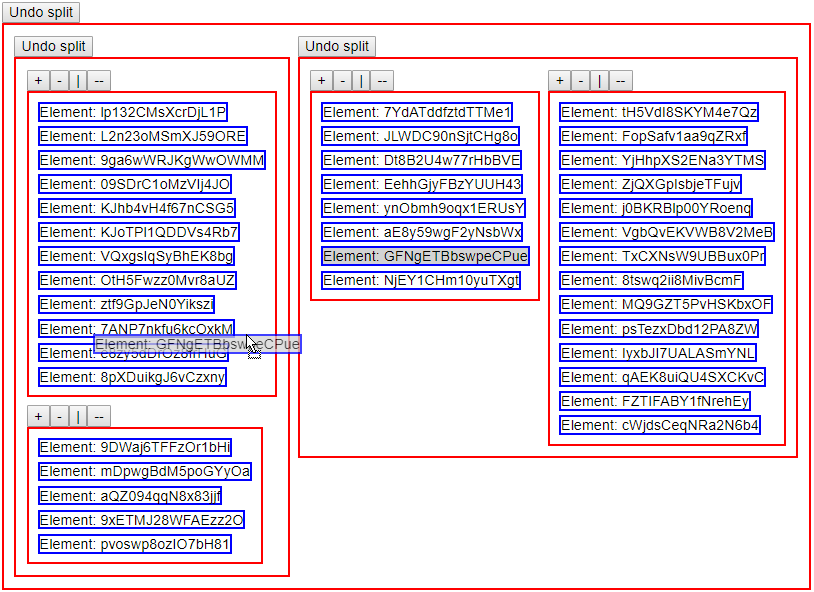
\includegraphics[width=0.8\textwidth]{figures/layout_grid_test.png}
        \caption{Eigener Layout-Prototyp mit CSS-Grids}\label{fig:layout_grid_test}
\end{figure}

\subsubsection{Umsetzung}\label{subsec:layout}
% table / grid

\subsection{Identifikation auf Server}
Um die UI-Elemente mit Daten aus der Datenbank zu befüllen muss eine entsprechende Identifikation möglich sein. Es wird vorausgesetzt dass diese eindeutige ID, ob sie aus Tabellennamen plus Spaltenname der Datenbank oder aus anderen Informationen besteht, zum Zeitpunkt der Übersetzung einer Ansicht bereits bekannt ist und mit ausgelesen werden kann. Bei Anfragen an den Server werden alle IDs der beteiligten Elemente mit an den Server übertragen, ebenso wie dieser bei Antworten immer die IDs der Elemente, für welche die Antwortdaten gedacht sind, sendet.

\subsection{Visualisierung von Lade- und Fehlerzustände}\label{subsec:loading_state_section}
Direktes Feedback ist für die subjektive Einschätzung einer performanten Webseite essentiell. Typischerweise ist die am längsten dauernde Aktion auf einer Webseite das Nachladen von Daten, es ist also sinnvoll diesen Vorgang für Nutzer visuell ansprechend deutlich zu machen. Für diesen Zweck sollen alle React-Komponenten eine visuell simplere Repräsentation von sich selbst in Form von unspezifischen grauen Boxen enthalten, welche nur auf die ungefähre Form und Darstellung mit Echtdaten hindeutet und die bereits während des Ladevorgangs angezeigt werden kann. In Abbildung~\ref{fig:comp_loading_final_comparison} sieht man eine Gegenüberstellung der beiden Repräsentationen (finaler Zustand links, Ladezustand rechts), jeweils für ein Edit-Element und ein Checkbox-Element.

\begin{figure}
    \centering
    \captionsetup{justification=centering}
    
\includegraphics[width=\textwidth]{figures/comp_loading_final_comparison.png}
        \caption{Ladezustand einer Komponente}\label{fig:comp_loading_final_comparison}
\end{figure}

Mit einer entsprechende Einfärbung und einem Hinweistext kann diese Visualisierung, wie in Abbildung~\ref{fig:comp_possible_error_state} an zwei unterschiedlichen Ausführungen gezeigt, ebenfalls dazu genutzt werden um Fehlerzustände beim Laden von Daten zu signalisieren.

\begin{figure}
    \centering
    \captionsetup{justification=centering}
    
\includegraphics[width=0.8\textwidth]{figures/comp_possible_error_state.png}
        \caption{Mögliche Fehlerzustände einer Komponente}\label{fig:comp_possible_error_state}
\end{figure}

\subsection{Einbindung von GraphQL mit Apollo}
Um \nameformat{Apollo} mit \nameformat{React} zu nutzen, muss zu Beginn einmalig die Adresse des Servers einer \textbf{Apollo-Provider}-Komponente übergeben werden. Diese umschließt alle weiteren Komponenten und dient dazu die Serveradresse an jeder Stelle der App zur Verfügung zu stellen. Zum Abfragen von Daten für die Darstellung in einer Komponente wird eine spezielle Funktion mit der \nameformat{GraphQL}-Abfrage, der daraus resultierenden Datenstruktur und der eigentlichen Komponente konfiguriert. Der Rückgabewert dieser Funktion verhält sich identisch zur übergebenen Komponente, enthält aber zusätzlich noch die aus der Abfrage erhaltenen Daten (und ggf. Lade- / Fehlerinformationen) als Übergabeparameter und kann diese identisch zu lokalen Daten bei der Anzeige nutzen.
Dieser Ansatz erlaubt es, die \nameformat{GraphQL}-Abfragen komponentenspezifisch (jede Komponente ist für den Aufbau der für sie notwendigen Abfrage zuständig) zu schreiben und lokal in einer zugehörigen Datei `<Komponentenname>.gql' zu speichern. Änderungen oder ein Austausch von Komponenten sind durch diese lose Kopplung der einzelnen Teile der Applikation trivial, da sie nur eine geringe Auswirkung auf alle anderen Komponenten haben.

\subsection{Unveränderbare Daten}
Das Verwalten von Mutationen mit veränderbaren Daten ist schwieriger, je größer ein Projekt wird, da diese immer in allen Teilen des Programms ausgeführt werden müssen. Durch Programmierfehler kann es passieren, das bestimmte Änderungen eventuell nicht überall vollzogen werden und so der State nicht mehr synchronisiert ist. Um diese Art von Fehler zu verhindern werden Daten nur an einer zentralen Stelle verwaltet (\textbf{single source of truth}) und sind an allen anderen Stellen unveränderbar (\textbf{immutable data}). Mutationen werden als Aktion an die für die Daten verantwortliche Stelle gesendet und nacheinander abgearbeitet.

\subsection{Editier-Modus}
In der UI angezeigte Daten kommen direkt vom Server und werden vor der Anzeige nicht weiter verarbeitet (siehe Abschnitt~\ref{subsec:api_client_no_business_logic}). Aufgrund dieser Tatsache kann eine Kopie des zu editierenden Objekts erstellt und Änderungen auf dieser Kopie ausgeführt werden. Wird der Editier-Modus durch Verwerfen der Änderungen beendet, so muss nur diese Kopie gelöscht werden. Andernfalls wird das Original durch die Kopie ersetzt und der Server über die Mutation benachrichtigt. Dieses Konzept wird von der Bibliothek \nameformat{immer.js} \parencite{weststrate_2019} umgesetzt und anhand einer Grafik (\ref{fig:immer_draft_concept}) sehr anschaulich dargestellt.

\begin{figure}
    \centering
    \captionsetup{justification=centering}
    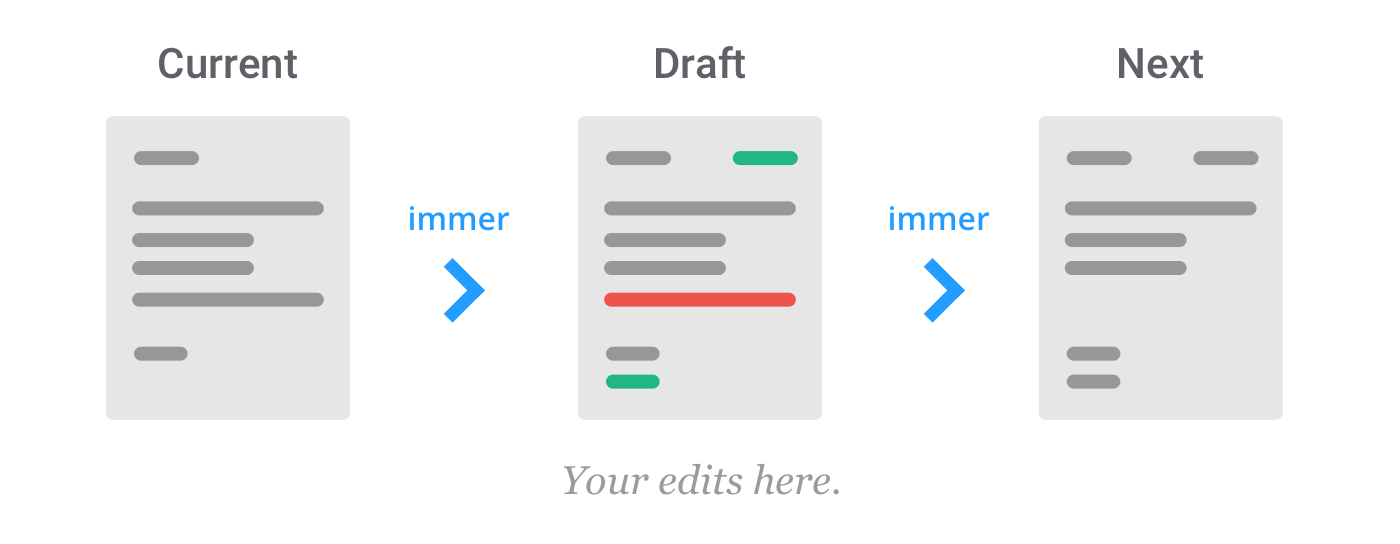
\includegraphics[width=\textwidth]{figures/immer_draft_concept.png}
        \caption{Editier-Konzept von immer.js \parencite{weststrate_2019}}\label{fig:immer_draft_concept}
\end{figure}

\subsection{Individualisierung}
Die Serialisierung des Layouts nach JSON geschieht über die jeweilige Darstellungsbibliothek der Ansicht. Zusätzliche (eigene) Formatierungen aus der Detailansicht werden anschließend im JSON ergänzt und dann auf den Server übertragen. Bevor das erste Mal eine solche Anpassung der Ansichten vorgenommen wird entspricht die Darstellung dabei der in Abschnitt~\ref{sec:ui_structure_translation} beschriebenen, aus der Desktop-UI automatisch generierten Struktur. Das Backend kann diese Informationen entweder direkt als Datei oder in einer NoSQL-Datenbank als Dokument abspeichern, oder seinerseits eine Serialisierung in bestehende SQL-Datenbankschemas vornehmen. Zur Darstellung werden diese Informationen wie in Abschnitt~\ref{subsec:grapql_schema} dargestellt wieder vom Server abgerufen.

\subsection{Suche, Filter, Sortierung}
Die Darstellung der Übersichtsliste wird, wie oben beschrieben, die \nameformat{React}-Bibliothek \nameformat{\fixme{name aus layout section oben}} (siehe Abschnitt~\ref{subsec:layout}) benutzt. Diese ermöglicht das Suchen, Filtern und Sortieren bereits ohne weitere Anpassungen. Für die Detailansicht müssen im jetzigen Stand analog zum Desktopclient die vorhandenen Möglichkeiten im Backend zur Umsetzung der Suche und Filter genutzt werden. Ein Nachteil dieses Ansatz ist natürlich, dass jedes Mal eine Anfrage an den Server geschickt werden und alle (gefilterten) Daten neu übertragen werden müssen. Eine bessere Alternative bestünde darin, die Daten der Detailansicht ebenfalls durch \nameformat{\fixme{name aus layout section oben}} verarbeiten zu lassen --- die technische Umsetzbarkeit bedarf weiterer Analysen der Bibliothek.

\subsection{Tests und Continuous Integration}
Boilerplate-Projekte welche mit dem \gls{cli}-Tool \nameformat{\gls{cra}} erstellt werden sind bereits so konfiguriert, dass gewöhnliche Tests (mit dem Testframework \nameformat{Jest}) direkt ausgeführt werden können. Entsprechende Tests sollen dabei entweder schon vor dem Hinzufügen neuer Funktionalitäten oder mindestens parallel dazu stattfinden. Zusätzlich wird noch die Bibliothek \nameformat{Enzyme} genutzt, welche React-Komponenten mit einer beliebigen Verschachtelungstiefe in eine Variable rendern und dadurch in Kombination mit Jest sogenannte Snapshot-Tests ausführen kann. Bei dieser Art von Test werden die Komponenten in eine JSON-ähnliche Struktur serialisiert und diese Struktur im Dateisystem gespeichert. Bei jeder weiteren Ausführung werden die alte und die neue Struktur miteinander verglichen und der Test als fehlgeschlagen gewertet, sobald die Strukturen Unterschiede enthalten. Mit dieser Art von Test kann sichergestellt werden, dass Änderungen an der Logik keine visuellen Artefakte generieren. Alle normalen und die beschriebenen Snapshot-Tests können im Sinne der kontinuierlichen Integration\footnote{CI: Continuous Integration} auf dem internen \nameformat{Team City}-Server ausgeführt werden.
Neben diesen Tests wird während der Entwicklung und Anpassung der UI das Tool \nameformat{Storybook} genutzt, mithilfe dessen eine React-Klasse isoliert von allen anderen Klassen angezeigt werden kann, genutzt. So ist es möglich, eine interaktive Echtzeit-Darstellung von Änderungen am Code zur direkten Beurteilung der gewünschten Auswirkungen zu nutzen.

\section{API}
\fixme{more infos?}

\subsection{Aufbau / GraphQL-Schema}\label{subsec:grapql_schema}
Das Schema, welches den Aufbau der Anfragen und damit gleichzeitig der Antworten vorgibt, enthält zwei Einstiegspunkte. Zum einen können Informationen zur Übersichtsliste und zum Anderen die der Detailansicht abgefragt werden. Beide Zweige sind weiterhin in eine Struktur- und einen Datenabschnitt getrennt. Clients können so zuerst die Struktur, also alle Enthaltenen UI-Elemente und deren Platzierung, Formatierung, etc., der Ansicht abfragen. Die reine Struktur enthält im Vergleich wenige Daten, eine entsprechende Abfrage erhält also zügig eine Antwort. Während die UI anschließend anhand der Struktur aufgebaut wird und Lade-Platzhalter (siehe Abschnitt~\ref{subsec:loading_state_section}) anzeigt können parallel die Daten nachgeladen werden. Sobald auch dieser Vorgang abgeschlossen ist werden die Lade-Platzhalter je nach Erfolg beziehungsweise Misserfolg mit den tatsächlichen Feldinhalten oder der Fehlervisualisierung inklusive Fehlermeldung ausgetauscht.

\subsection{Keine Business Logik im Client}\label{subsec:api_client_no_business_logic}
Clients sollten keine eigenen Schlussfolgerungen aus den von der API gelieferten Daten ziehen müssen. Dies ist ein häufig begangener Fehler, bei dem die API Daten zu einer Ressource angibt, diese Daten aber nicht direkt angezeigt sondern erst noch auf irgendeine Art verarbeitet und transformiert werden müssen. Es kann vorkommen, dass verschiedene Implementierungen von Clients an dieser Stelle andere Transformationen anwenden und die sichtbare Darstellung dabei für Endanwender inkonsistent erscheint. Selbst wenn darauf geachtet wird, dass zu einem Zeitpunkt X alle Clients konsistent implementiert sind ist es möglich diese Konsistenz durch Bugfixes oder andere clientspezifische Anpassungen in der Zukunft zu einem beliebigen Zeitpunkt Y wieder zu verlieren. Ein Beispiel für einen solchen Fall, beschrieben von Phil Sturgeon \parencite{sturgeon_2017}, ist eine API die Anfragen über Rechnungen beantwortet und dabei verschiedene Felder liefert. Enthält das Feld `\textbf{bezahlt-am}' keine Daten, können Clients davon ausgehen dass die Rechnung noch nicht bezahlt wurde. Wenn nun ein weiteres Feld, welches anzeigt ob der Betrag tatsächlich auf dem Empfängerkonto eingegangen ist, `\textbf{bezahlung-erhalten-am}' hinzugefügt wird, zeigen alte Clients den Status weiterhin als `Bezahlt', sobald das erste Feld einen Wert enthält. Clients die ein Update erhalten haben zeigen dieses Status jedoch erst, wenn beide Felder einen Wert enthalten.
Entsprechend ist diese API so konzipiert, dass notwendige Transformationen immer im Backend vollzogen werden. In der aktuellen Implementierung gibt es noch keine Instanz bei der dieses Paradigma angewendet werden muss, spätere Anpassungen und Ergänzungen an der API müssen aber entsprechend umgesetzt werden.

\chapter{Implementierung eines Prototypen}
\label{chap:implementation}

In diesem Kapitel wird die Entwicklung eines auf dem zuvor ausgearbeiteten Konzept basierten Prototypen beschrieben. Dieser Prototyp enthält nicht alle im Konzept beschriebenen Anforderungen und befindet sich auch nicht in einem finalen Entwicklungsstadium, kann aber mit weiteren Entwicklungsressourcen als Grundlage für eine finale Implementierung genutzt werden. Er soll zeigen, wie sich das entworfene Konzept umsetzen lässt und die darin benutzten Technologien miteinander interagieren.

\section{Tool zum Parsen der vorhandenen UI-Persistierung}

Wie in Kapitel~\ref{chap:concept} beschrieben müssen die Dateien welche das momentane UI-Layout enthalten in ein web-freundlicheres Format (JSON) übersetzt werden. Bei diesem Schritt ist es auch direkt möglich Informationen die zukünftig nicht mehr benötigt werden nicht mit zu übernehmen und andere Informationen in eine optimalere Struktur zu überführen. Für diesen Zweck wurde ein kleines Hilfstool in C\# geschrieben, welches sowohl die ``.dli''-Datei der Detailansicht als auch die ``.vlc''-Datei der Übersichtsliste einer einzelnen cRM-Ansicht als Input erhält und daraus eine ``.json''-Datei mit allen benötigten Informationen erstellt. Um die Anpassbar- und Wiederverwendbarkeit des Tools zu maximieren wurde das Visitor-Pattern \fixme{Erklärung?} angewandt. In Abbildung \ref{fig:web-conv_file-tree} ist der Aufbau des Tools erkennbar.

\begin{figure}
    \centering
    \captionsetup{justification=centering}
    \frame{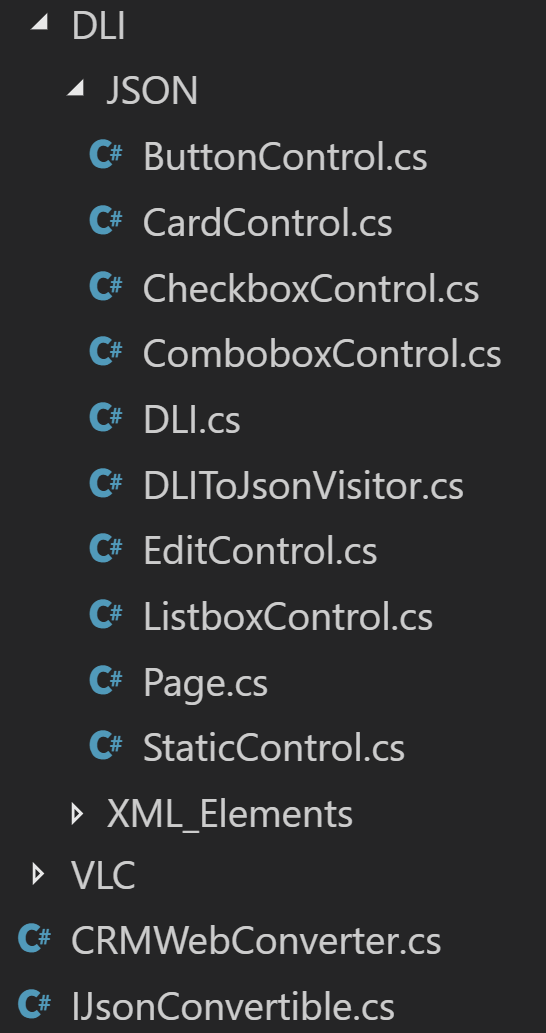
\includegraphics{figures/web-converter_file-tree.png}}
        \caption{Datei-Struktur des Konvertierungstools}
        \label{fig:web-conv_file-tree}
\end{figure}

Zunächst wird für jedes einzulesende Token (XML-Element) eine eine Klasse vom ``Acceptor''-Interface (IDLIAcceptor / IVLCAcceptor) abgeleitet, dieses Interface enthält eine einzige Methode ``Apply'', welche einen Visitor (IDLIVisitor / IVCLVisitor) übergeben bekommt. Die jeweiligen Token-Klassen werden mit dem von ihnen verwalteten XML-Element (XElement) initialisiert. Wie im Quellcodeauszug \ref{lst:pageelement_init} anhand der Klasse ``PageElement'' beispielhaft zu sehen werden aus diesem XML-Element die relevanten Informationen über das Element selbst (Name und Metadaten) und dessen verschachtelte Kinder-Elemente (Liste von Controls) ausgelesen.

\lstinputlisting[language={[Sharp]C},label={lst:pageelement_init},caption={Initialisierung der PageElement-Klasse}]{code/chapter_005_pageelement_init.cs}

\fixme{syntax highlights}
Nachdem die Informationen der XML-Datei auf diese Art und Weise in ihre einzelnen Token-Instanzen übersetzt wurden wird die Apply-Methode, zu sehen in Quellcodeauszug \ref{lst:dialogelement_apply}, des zentralen Tokens (DialogElement) mit einer Visitor-Instanz aufgerufen. Der Visitor erhält als Parameter eben diese Instanz und extrahiert alle für ihn relevanten Informationen. Anschließend ruft er rekursiv die Apply-Methoden der Kinder-Token auf und liest auch aus diesen die relevanten Informationen aus. Diese Aufrufe sind im Quellcodeauszug \ref{lst:json-visitor_visit-methods} zu sehen. Nachdem alle Tokens vollständig besucht wurden können die gewonnenen Daten als JSON-String ausgegeben werden.

\lstinputlisting[language={[Sharp]C},label={lst:dialogelement_apply},caption={Apply-Methode der DialogElement-Klasse}]{code/chapter_005_dialogelement_apply.cs}

\lstinputlisting[language={[Sharp]C},label={lst:json-visitor_visit-methods},caption={Besuchen von und Extrahieren relevanter Informationen aus XML-Tokens durch den JSON-Visitor}]{code/chapter_005_json-visitor_visit-methods.cs}

Die Flexibilität dieser Architektur, welche in der Abbildung \ref{fig:web-conv_class-diagramm} nochmals übersichtlich als Klassendiagramm dargestellt wird, ist ebenso daran zu erkennen, dass der einzige Unterschied beim Auslesen von Detailansicht-Datei und Übersichtslisten-Datei in der Implementierung der Interfaces besteht. Sowohl Acceptor- \fixme{some kind of highlight, italize?} als auch Visitor-Klassen können sehr leicht einzeln angepasst oder ersetzt werden. Ebenso ist es möglich weitere Tokens, welche eventuell zu einem späteren Zeitpunkt benötigt werden, aus den XML-Dateien auszulesen, indem man weitere Acceptor- und Visitor-Implementierungen hinzufügt.

\begin{figure}
    \centering
    \captionsetup{justification=centering}
    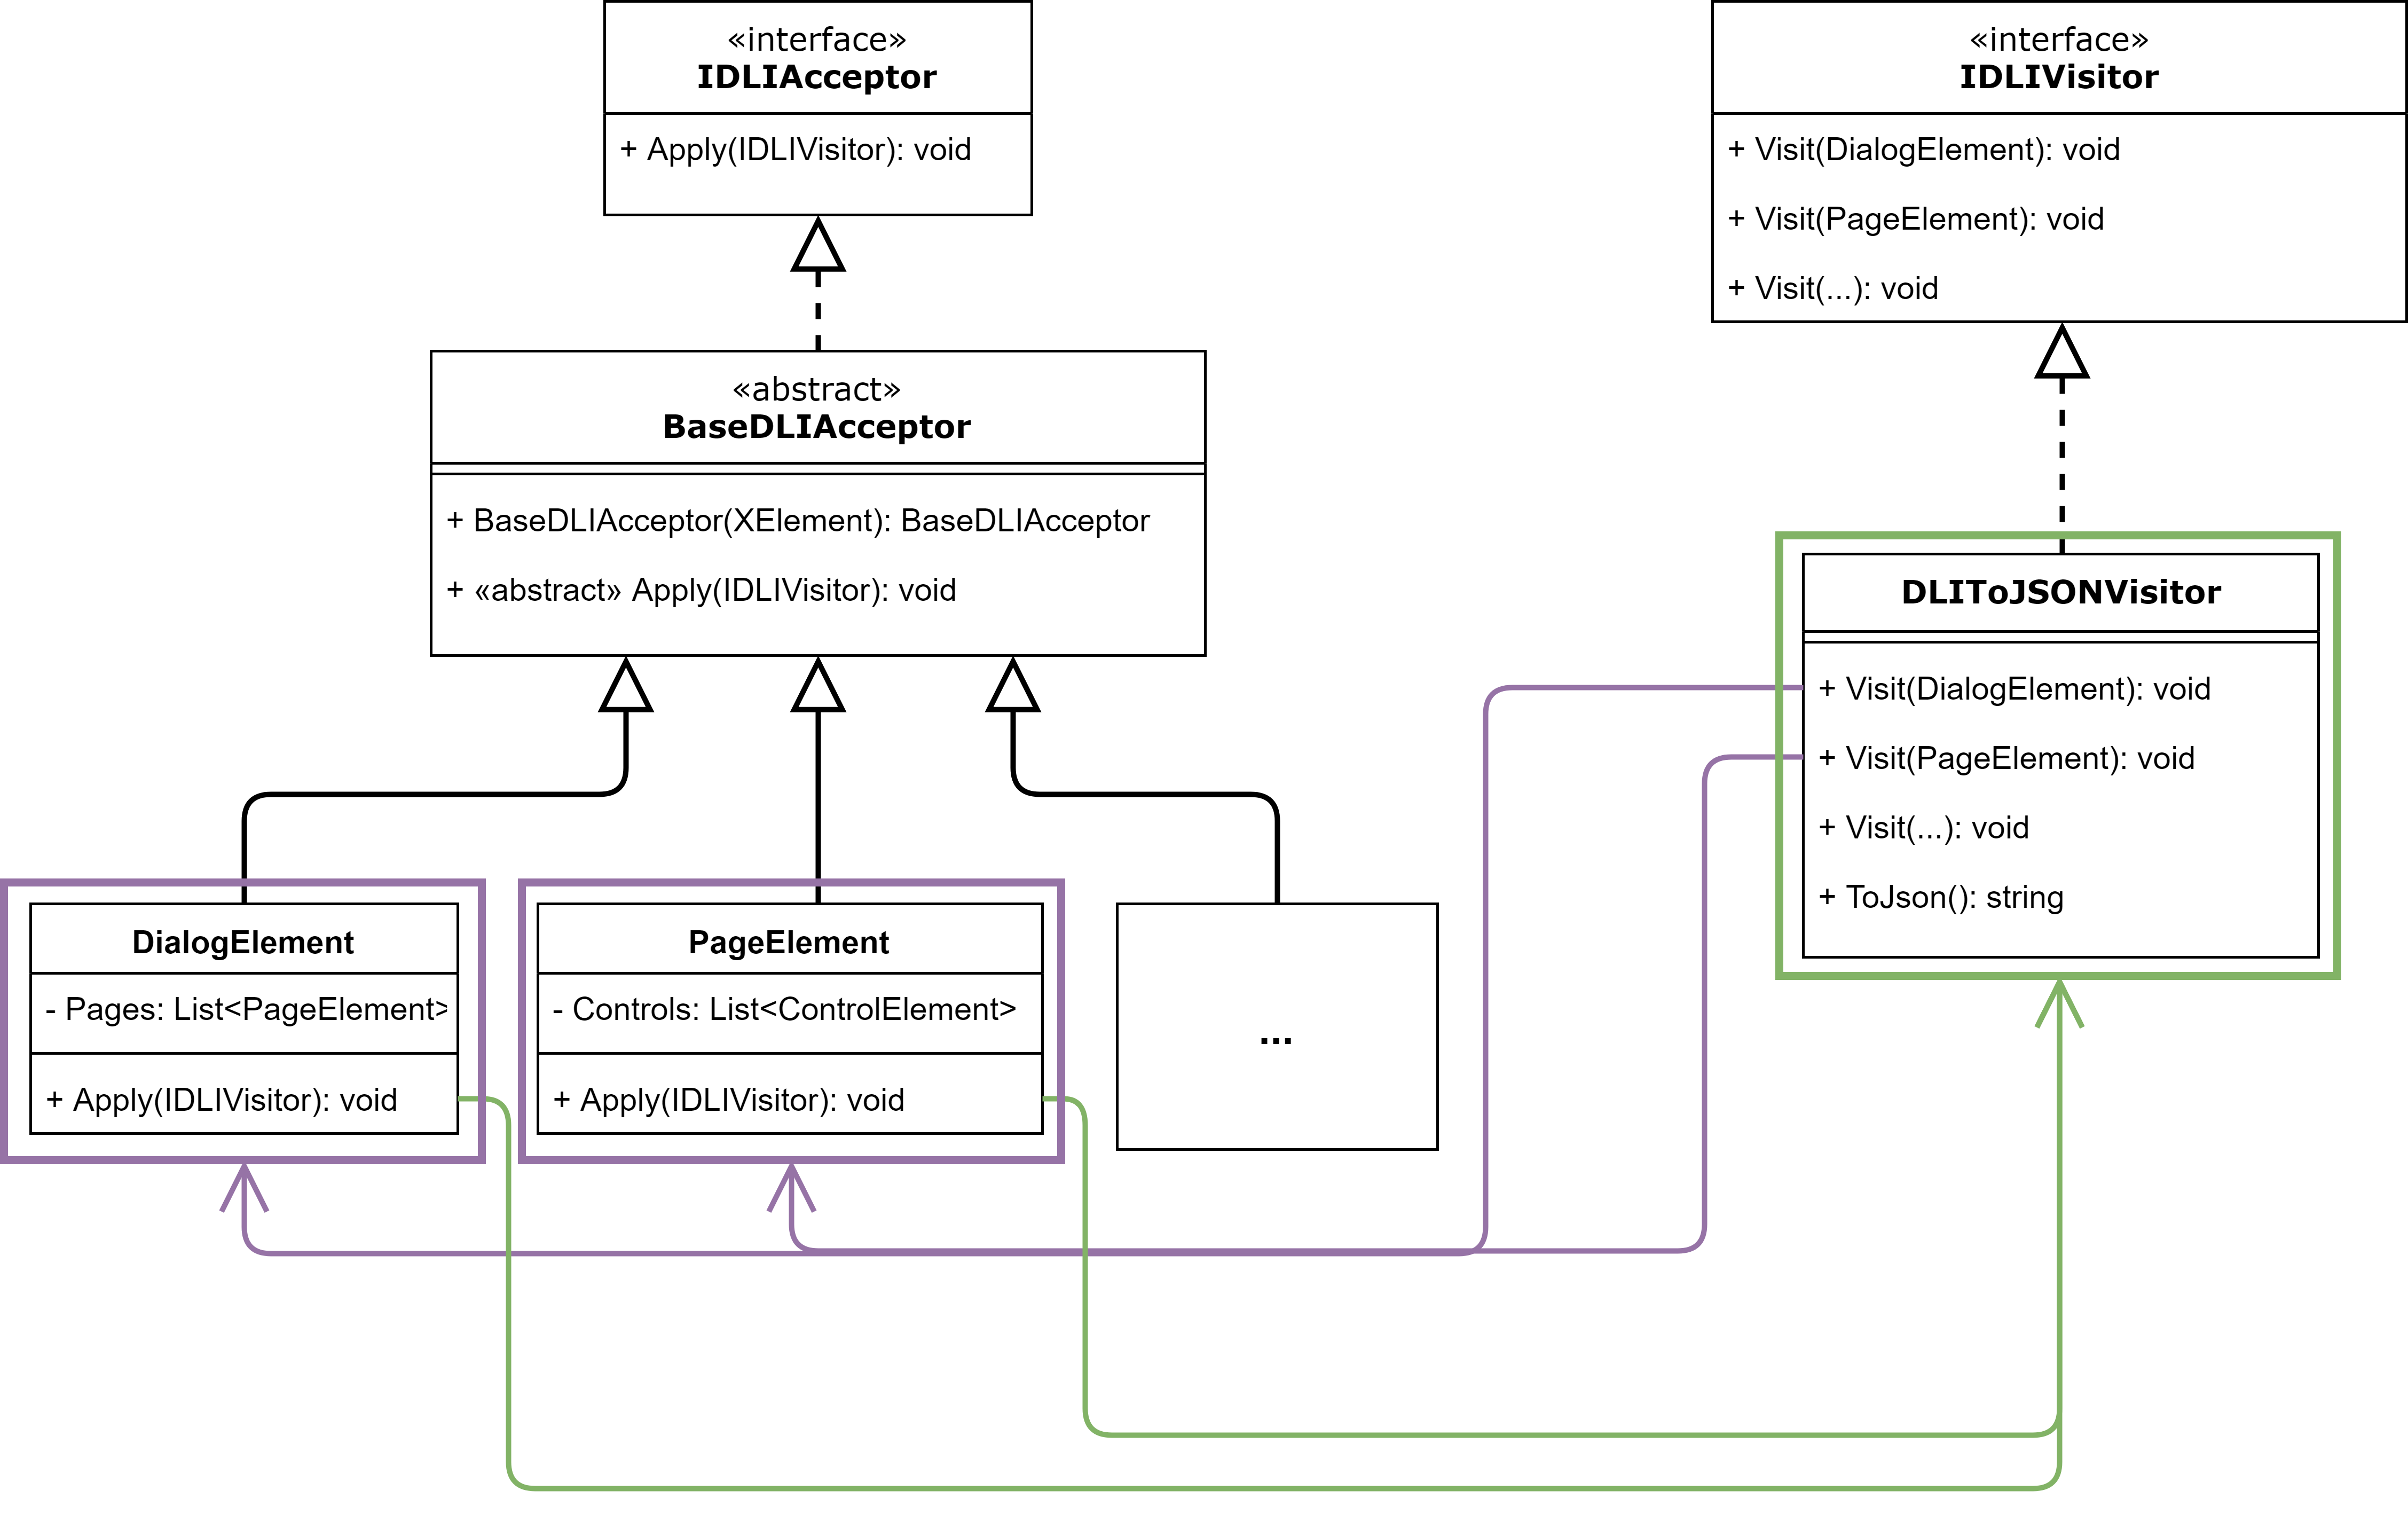
\includegraphics[width=\textwidth]{figures/web-converter_class-diagramm.png}
        \caption{Klassendiagramm der Visitor-Struktur des Konvertierungstools}
        \label{fig:web-conv_class-diagramm}
\end{figure}

Der Input und das Endergebnis in Form eines vom GraphQL-Server direkt verwertbaren JSON-Dokument ist in den beiden Quellcodeauszügen \ref{lst:xml_input} und \ref{lst:json_output} anhand eines kleines Auszuges ersichtlich. \fixme{vollständigeres beispiel und erklärung?}

\begin{minipage}{.5\textwidth}
    \lstinputlisting[language={XML},caption={XML-Input},label={lst:xml_input}]{code/chapter_005_xml_input.xml}
\end{minipage}\hfill
\begin{minipage}{.4\textwidth}
    \lstinputlisting[caption={JSON-Ergebnis},label={lst:json_output}]{code/chapter_005_json_output.json}
\end{minipage}    

\section{Webseite}

\subsection{CRA-Skelett}
\subsection{Benutzung der vorgefertigten UI-Elemente}
\subsection{Storybook und Tests}
\subsection{GraphQL-Mock-Server und Resolver}

\chapter{Fazit}

%% Use letters for the chapter numbers of the appendices.
\appendix{}

%\input{appendix_a}

\printbibliography[title=Quellenverzeichnis, heading=bibintoc]

\end{document}
